%----------------------------------------------------------------------------------------
%	PACKAGES AND OTHER DOCUMENT CONFIGURATIONS
%----------------------------------------------------------------------------------------


\documentclass[12pt,openright,twoside,final]{report}
% PACKAGES
\usepackage{multirow}
\usepackage{generators/imports}
\usepackage{hyperref} %for inserting hyperlinks
%\hypersetup{
%    colorlinks=true,
%    linkcolor=blue,
%    filecolor=magenta,      
%    urlcolor=cyan,
%}
\usepackage{tikz}
\usepackage{amsthm} % for proofs
\usetikzlibrary{positioning}
\usetikzlibrary{decorations.text}
\usetikzlibrary{decorations.pathmorphing}

\makeglossaries

\renewcommand*{\acronymname}{List of Acronyms and Abbreviations}
\renewcommand{\glsnamefont}[1]{\textbf{#1}}

%Create acronyms here.
\newacronym{saas}{SaaS}{Software as a Service}
\newacronym{kg}{KG}{Knowledge Graph}
\newacronym{vcs}{VCS}{Version Control System}
\newacronym{rdfs}{RDFS}{Resource Description Framework Schema}
\newacronym{w3c}{W3C}{World Wide Web Consortium}
\newacronym{dl}{DL}{Description Logic}
\newacronym{una}{UNA}{Unique Name Assumption}
\newacronym{owl}{OWL}{Web Ontology Language}
\newacronym{rnn}{RNN}{Recurrent neural network}
\newacronym{fol}{FOL}{First Order Logic}
\newacronym{pl}{PL}{Propositional Logic}
%You can also do explanations.
\newglossaryentry{git}{name={Git},
    description={Git is a \gls{vcs} for tracking changes in computer files and coordinating work on those files among multiple people}}

\begin{document}
\include{generators/frontpage} % This is the titlepage
\pagenumbering{roman}
%\cite{schlichtkrull2018modeling, vashishth2019composition} (for neural networks citation)
\begin{abstract} 

\noindent Knowledge graphs (KGs) have risen in both size and use over the past few years, and there are a range of approaches for evaluating information in them. Symbolic approaches, such as rule-based machine learning, offer an explainable way to determine the appropriateness of a new fact based on rules mined from the KG in question. Some of the most successful approaches for fact prediction in KGs today are knowledge graph embeddings (KGEs) that use deep neural networks, however, these lack the explainability of symbolic approaches. We would like to see how the extension of a KG using KGEs affects the rules mined from the KG. A set of rules is mined from a KG and compared with another set mined from an \textit{extended} version of said KG. The experiments examine three classical KGEs: TransE, DistMult, and ComplEx, and use the rule mining algorithm AMIE3. AMIE3 is treated as a black box during the experiment, as the study only evaluates factors playing a role in the KG-extension process, one of which is the choice of KGE. The experiments show that there can be considerable discrepancies in the rules mined based on the choice of KGE and that TransE leads to a substantial amount of nonsensical rules being mined.

\end{abstract}

\renewcommand{\abstractname}{Acknowledgements}
\begin{abstract}
    First and foremost, I would like to thank my two supervisors, Ana and Ricardo. Ana was, from the start, a fantastic guide for me in the field of academic research and taught me a lot about writing and publishing work. Ricardo was always eager to answer and discuss questions, and his attention to detail taught me a lot. A great thank you to both of you. You have given me more support through this master's than I could have hoped for.
	
	I would like to thank my fellow master's students that battled with me over the two years. The workload is not so heavy when you are in it together. Thank you John Isak, Hans Martin, Knut, Halvor, Mathias, Magnus, Emir and Oda. You have been a fantastic group to work with, and I wish you all the best in your future work/studies.
	
	My final thanks goes out to family and friends, who have helped me by listening to my thoughts and reviewing the thesis. Complicated ideas become tangible and manageable when you put the correct words to them. Thank you for helping me find them.
	
	\vspace{1cm}
	\hspace*{\fill}Johanna Jøsang\\ 
	\hspace*{\fill} 01 June, 2022
\end{abstract}
\newpage
\include{generators/tableOfContentsAndListings}
\pagenumbering{arabic}
\setcounter{page}{1}
\setlength{\parskip}{0.5cm plus4mm minus3mm}  

\chapter{Introduction}
\section{Context and motivation}
\Glspl{kg} are an increasingly popular way to represent data \cite{hogan2020knowledge}.
A \gls{kg} are often seen as a directed graph with labelled edges where the nodes represent the elements in a domain of interest (e.g. people), and the edges represent a relation between two elements. For instance, a \gls{kg} such as Wikidata might include the node ``Oslo'' with an outgoing edge labelled ``capital of'' to the node ``Norway''. Knowledge graphs that are large and interesting are generally not complete. They may, for example, be extracted from natural language resources and may contain facts that are wrong or exhibit gaps in their knowledge. However, most of the present data is typically correct and implicitly contains meaningful rules. For example, Wikidata will implicitly contain the rule that siblings tend to have the same mother:
\[has\_sibling(x, z) \wedge has\_mother(z, y) \Rightarrow has\_mother(x, y)\]
There will of course be exceptions to this rule, but generally, it will hold. Such a rule can be used to infer new information in a \gls{kg}, and using a set of such rules to make predictions is the core idea behind rule-based machine learning. Other statistical methods are accurate and scalable when it comes to inferring new facts from \glspl{kg}, but one of the main issues of these approaches is that results usually are not explainable \cite{bonatti2019knowledge}. Rule-based machine learning approaches, on the other hand, provide an explanation in the form of the rules used to make a prediction. Meilicke et al. showed that rule bases mined with the AMIE+ algorithm are good competitors and often outperform vector embedding models \cite{ensemble}. One explanation for this is that the standard benchmark datasets, such as WN18 and FB15k,  have many relational regularities, such as symmetry and equivalence. Meilicke et al. also compared the two approaches for triple prediction and found that they complement each other. An ensemble of the two families of methods gave better results than either of the two alone.

This work by Meilicke et al. inspired the idea of using \gls{kge} models to improve rule bases or vice versa. The idea is to use one technique to ``extend" the original \gls{kg} and thereafter train the second one on the extended \gls{kg}. The \gls{kg}-extension-and-mining pipeline can be done both ways, as shown in figure \ref{rule_based_and_embedding}. A rule-base as the end result was chosen, ultimately because it results in an explainable model.

\begin{figure}[H]
    \centering
    \includesvg[inkscapelatex=false,width=1\textwidth,keepaspectratio]{figures/intro/custergraf-nesten.svg}
    \caption[Figure representing the process.]{The two versions of \gls{kg} improvement for better model creation. In the top version, an embedding of the original \gls{kg} is used to improve the graph, from which a rule base is mined. Red edges represent new links made by the models, which originally weren't present in the \gls{kg}. The bottom half of the figure describes the same process but with the rule base used to improve the \gls{kg}, resulting in an embedding of the improved \gls{kg}.}
    \label{rule_based_and_embedding}
\end{figure}

\section{Research questions}
With this idea in mind, the general question to be explored is what role different factors in the \gls{kg} extension process have on the eventual rules that are mined from the extended dataset. The extension process can be summarized as follows: first, candidate facts are generated, then an embedding model ranks the candidates, and finally facts above a certain threshold are added to the \gls{kg}. So the factors to be evaluated are:
\begin{itemize}
    \item How candidate facts are generated.
    \item How candidates are ranked (choice of \gls{kge} model).
    \item What minimum rank candidates must have to be added to the \gls{kg}.
\end{itemize}

In addition to evaluation of these parameters, the current work explores three central research questions:
\begin{enumerate}
    \item Does adding new plausible facts lead to new rules being mined?
    \item How does the quality (approximated with PCA confidence) of new rules compare to the rules mined from the original \gls{kg}?
    \item Can the rules mined from the original \gls{kg} also be mined after the \gls{kg} is extended?
\end{enumerate}

To answer these questions, the mentioned \gls{kg}-extension-and-mining pipeline is implemented and the results evaluated. Experiments are conducted on two different datasets, both of which are commonly used for benchmarking \glspl{kge}. The most important results of this work are presented in a paper submitted to this year's \href{https://sites.google.com/view/kr4hi/home}{\textit{International Workshop on Knowledge Representation for Hybrid intelligence}}. The submission can be accessed through this link: \href{https://1drv.ms/b/s!AmqWMjPoErw-lIMSvmZOPIGrHn4l-g?e=MYpkuS}{OneDrive}.

%The thesis examines whether adding new plausible facts will lead to new rules being mined and how the quality (approximated with PCA confidence) of these rules compares to that of the rules mined from the original \gls{kg}.

%The rules describe information about relational data, and hence will only use binary predicates. The rules will also be Horn, meaning that any number of predicates may be used in the body of the rule, but only one predicate is implied in the rule. This form has useful properties in knowledge representation and reasoning. When extracting rules from knowledge graphs they therefore tend to be Horn rules on binary predicates.


\section{Thesis outline}
The outline for the rest of the thesis is as follows: \newline \newline
\textbf{Chapter 2 - Background} provides the reader with the background knowledge required for a proper understanding of the work. \newline
\newline
\textbf{Chapter 3 - Rule mining on extended knowledge graphs} explains the methodology and material used for experiments. \newline
\newline
\textbf{Chapter 4 - Results} presents and discusses the findings of the experiment. \newline \newline
\textbf{Chapter 5 - Related work} provides the reader with an overview of works related to the thesis. \newline \newline
\textbf{Chapter 6 - Discussion} evaluates and discusses the current work and explains an earlier approach explored during research.
\newline \newline

As a final note, this thesis assumes that the reader is familiar with basic machine learning concepts, such as training, testing and overfitting. For an introduction or refresher to machine learning basics, chapter 5 in the book \textit{Deep Learning}, by Goodfellow et al. \cite{goodfellow} covers the topic quite well. The entire book is publicly available at \href{https://www.deeplearningbook.org/}{https://www.deeplearningbook.org/}.
\chapter{Background}

This chapter presents knowledge graphs and different paradigms for how to interpret information missing from a KG. Then we continue with knowledge graph embeddings where we examine the training and evaluation process and explain the ideas behind the three knowledge graph embedding architectures used in the experiments. Finally, the chapter introduces rule mining by first giving a general overview of rule-based machine learning before focusing on the \textit{association rule mining} approach.

\section{Knowledge Graphs}
There is no single agreed upon definition of \glspl{kg} \cite{bergman_2019, bonatti2019knowledge, ehrlinger2016towards}. Definitions and usages vary from specific technical proposals to more general descriptions. In this thesis, we will use the more inclusive definition similar to the one proposed by Hogan et al. \cite{hogan2020knowledge}, where we view a \gls{kg} as \textit{a graph of data intended to capture the semantic connections within real world knowledge, where nodes represent relevant entities and edges represent relations between these entities}. The type of graph may vary, i.e. it may be simple, directed, etc. A graph may contain knowledge over a broad range of domains, such as Wikidata~\cite{lehmann2015dbpedia}, or be limited to a specific domain, such as DBpedia \cite{fellbaum2010wordnet}. The concept of ``knowledge'' has been widely debated in epistemology \cite{chappell2005plato, kirkham1984does, wittgenstein1969certainty, gottschalk2008internet}, but here we will use it to mean descriptive knowledge, meaning facts that can be stated. Knowledge can be simple statements, such as ``\textit{Leo is a cat}'', or quantified statements such as ``\textit{at least one cat is black}''. %KGs are not expressive enough for quantified statements, where ontologies or rules would be more appropriate. 
Additional knowledge can be inferred from KGs through inductive or deductive methods. For example from a KG containing the information that ``\textit{Leo is a cat}'' and ``\textit{cats are mammals}'', one can deductively infer that ``\textit{Leo is a mammal}''. If all cats mentioned in the knowledge graph like to eat fish, then one can inductively infer ``\textit{cats like to eat fish}''.

\begin{figure}[htbp]
\centering
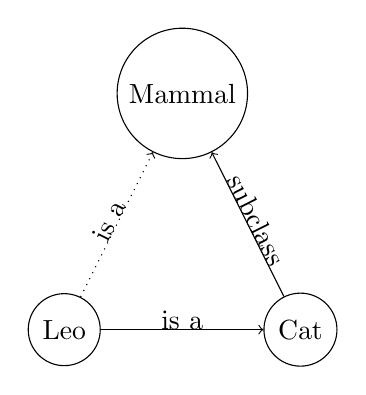
\begin{tikzpicture}
    \node[shape=circle,draw=black] (L) at (0,0) {Leo};
    \node[shape=circle,draw=black] (C) at (3,0) {Cat};
    \node[shape=circle,draw=black] (M) at (1.5,3) {Mammal};

   % \path [->] (L) edge node[left] {$IsA$} (C);
   \draw [->] (L) -- (C);
   \draw [decoration={text along path,
    text={is a},text align={center}},decorate]  (L) -- (C);
    
    \draw [->] (C) -- (M);
   \draw [decoration={text along path,
    text={subclass},text align={center}},decorate]  (M) -- (C);
    
    \draw [dotted, ->] (L) -- (M);
   \draw [decoration={text along path,
    text={is a},text align={center}},decorate]  (L) -- (M);
    
\end{tikzpicture}

\caption[Simple visual example of a KG.]{Example of a KG, where the dotted line represents a relationship that can be deductively inferred.} \label{fig:KGexample}
\end{figure}

In this thesis we will loosely follow the Resource Description Framework (RDF) standard and view KGs as sets of semantic triples. RDF is a standard for representation and exchange of graph data introduced by \gls{w3c}. Semantic triples are the data types used in the RDF data model. A triple, as the name suggests, is a tuple of three elements. It has the form (subject, predicate, object) and can therefore represent statements about semantic data, for example ``\textit{Cats are mammals}", or ``\textit{Ann knows Bob}". These RDF statements express relationships between two web resources, these resources being the subject and the object, while the predicate encapsulates the nature of the relationship. The relationship is phrased in a directional way, and so a set of RDF statements can also be viewed as a directed graph. The graph represents these triple statements, where the predicate in the triple denotes the edge going from the subject to the object, both of which are vertices.

\begin{lstlisting}[caption={Example of RDF triple set written in informal pseudocode.}, label={RDF_triples_example}]
<Leo> <is a> <cat>
<cat> <is a> <mammal>
<Ann> <knows> <Bob>
<Ann> <is a> <person>
<Bob> <is a> <person>
<Ann> <has pet> <Leo>
\end{lstlisting}

\begin{figure}[htbp]
\centering
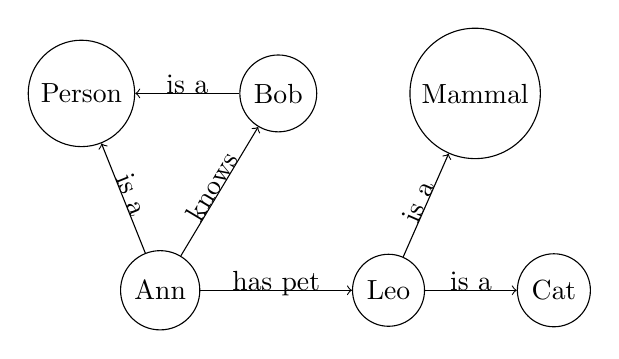
\begin{tikzpicture}
    \node[shape=circle,draw=black] (L) at (3.9,0) {Leo};
    \node[shape=circle,draw=black] (P) at (0,2.5) {Person};
    \node[shape=circle,draw=black] (A) at (1,0) {Ann};
    \node[shape=circle,draw=black] (B) at (2.5,2.5) {Bob};
    \node[shape=circle,draw=black] (C) at (6,0) {Cat};
    \node[shape=circle,draw=black] (M) at (5,2.5) {Mammal};

   % \path [->] (L) edge node[left] {$IsA$} (C);
   \draw [->] (L) -- (C);
   \draw [decoration={text along path,
    text={is a},text align={center}},decorate]  (L) -- (C);
    
    \draw [->] (L) -- (M);
   \draw [decoration={text along path,
    text={is a},text align={center}},decorate]  (L) -- (M);
    
    \draw [->] (A) -- (B);
   \draw [decoration={text along path,
    text={knows},text align={center}},decorate]  (A) -- (B);
    
    \draw [->] (A) -- (L);
   \draw [decoration={text along path,
    text={has pet},text align={center}},decorate]  (A) -- (L);
    
    \draw [->] (A) -- (P);
   \draw [decoration={text along path,
    text={is a},text align={center}, reverse path},decorate]  (A) -- (P);
    
    \draw [->] (B) -- (P);
   \draw [decoration={text along path,
    text={is a},text align={center}, reverse path},decorate]  (B) -- (P);
    
\end{tikzpicture}

\caption[Visualization of RDF triple example in listing \ref{RDF_triples_example}]{Informal visualization of the KG consisting of the example triples from Listing \ref{RDF_triples_example}} \label{fig:KG_example_2}
\end{figure}

With this type of data organisation one can for example query for a list of all people who own cats in the dataset. Treating KGs as a set of triples is the data model used in this thesis.

\subsection{Integrity of KGs}
\label{Integrity_of_KGs}
Generally, KGs contain only true facts. As with all databases, there is seldom a use in documenting all things that are not true. By the \textit{closed world assumption } (CWA) all facts not present in the KG are considered false. For example, by the KG in figure \ref{fig:KG_example_2} the statement \texttt{<Ann> <has sibling> <Bob>} is false under the CWA, as it is not present in the KG. So under the CWA Bob is not a sibling of Ann. The \textit{open world assumption} (OWA) makes no such claims and  the validity of a triple not present in the KG is considered unknown. In the above example, Bob is therefore neither considered a sibling of Ann nor not a sibling of Ann under the OWA.

In the context of KGs the OWA is often more justified, as most large interesting KGs are far from complete. For example, the KG Wikidata5M does not contain information about the national bird of countries. This of course does not make the statement ``\textit{The kiwi is the national bird of New Zealand}" any less true. The information has simply not been included in the KG. Another example is Freebase, the precursor to Wikidata, in which 70\% of people listed had the place-of-birth attribute missing \cite{west2014knowledge}.

\begin{figure}[htp]
    \centering
    \includegraphics[width=10cm]{figures/kb_venn.png}
    \caption{KB prediction under incompleteness.}
    \label{KB_predictions}
\end{figure}

The OWA has a central problem regarding machine learning; it fails to provide counterexamples. Because missing facts are assumed to be neither true nor false, there are no false facts to give as examples when mining rules or training an embedding model. We used figure \ref{KB_predictions}, similar to the one used in the paper introducing AMIE \cite{amie}, to aid the explanation of solutions to this problem. The figure represents all possible triples given the relation $r$ and entities in a KG. These triples can be split into four types:
\begin{enumerate}
    \item KG true: True facts in the KG
    \item NEW true: True facts not in the KG
    \item KG false: False facts \textit{known to} the KG
    \item NEW false: False \textit{unknown to} the KG
\end{enumerate}
When considering false facts we use the words ``\textit{known}" and ``\textit{unknown}" as a KG generally does not contain false triples. We consider a given rule $B \Rightarrow r(x, y)$, where $B$ denotes the body of the rule and $r(x, y)$ the consequent. In figure \ref{KB_predictions} the red circle denotes predictions made by this rule. These predictions can be true and in the KG (A), true and outside the KG (B), false and known to be false (C) or false and unknown to be false (D). 

In the context of the predictions of the rule, we want to maximize B over D. Under the OWA, however, there are no false facts, so we don't know what B and D are. The authors of AMIE therefore introduced a new paradigm called the \textit{partial completeness assumption} (PCA) \cite{amie}. It assumes that if $r(x, y) \in KB true$ for some entities $x$, $y$, then
\[\forall y' : r(x, y') \in KBtrue \cup NEWtrue \Rightarrow r(x, y') \in KBtrue\]
, where $x$ is the \textit{head} of the triple (the first variable in the binary predicate) and $y$ is the \textit{tail} of the rule (the second varaible in the binary predicate).
This assumption says that if the KG already has $r$-related information about the entity $x$,  then it contains \textit{all} $r$-related information about $x$. For example if a KG only contains \texttt{<Ann> <has sibling> <Bob>} and no other sibling entries with Ann as the head, then by the PCA Bob is Ann's only sibling. All other facts claiming that Ann has other siblings will therefore be negative examples. If we then however ask what \textit{friends} Ann has in a knowledge base without information about Ann's friends, then one cannot conclude that Ann is friendless. PCA is a more particular version of the broad \textit{partial-closed world assumption} (PCWA), where the KG generally is treated under the OWA, but parts of it that are considered complete are treated under the CWA \cite{motro1989integrity}. The PCA is particular in the sense that it specifically defines what parts of the KG should be treated under closed-world semantics.

\section{Knowledge Graph Embeddings}
\label{KG_embeddings}
Let $\mathcal{K}$ be a KG with triples of the form $(h, r, t)$ with $r\in \mathbb{P}$ and $h, t \in \mathbb{E}$, where $\mathbb{P}$ and $\mathbb{E}$ are respectively the set of all relations and the set of all entities entities in $\mathcal{K}$. Entities and relations are embedded in a vector space. To simplify the explanation we let the dimension of both entities and relations in the embedding space to be $d$.
Given $\mathcal{K}$ and $d$, a KG embedding seeks to represent all entities and relations in the continuous vector space of $d$ dimensions. These representations are meant to capture the semantic information in the graph. An embedding that manages this can then be used to evaluate the probability of new triples being true in the context of the KG and identify false information in $\mathcal{K}$.%, two tasks respectively called \textit{link prediction} and \textit{triple classification}.

\begin{figure}[htp]
    \centering
    \includesvg[inkscapelatex=false,width=1\textwidth,keepaspectratio]{figures/KG_embeddings/KG_embedding_diag.svg}
    \caption[KG embedding process.]{KG embedding process. Them embedding of a KG can be used for machine learning tasks. Figure is based on work by Edoardo Ramalli \cite{wiki_KG_embedding}.}
    \label{KG_embdding_diag}
\end{figure}

TODO: talk about training and overfitting \newline
The procedure for training KG embedding models is similar to any other statistical-based machine learning. The values of the embeddings are usually initialized as random values. These embeddings are continuously optimized through a training loop, which stops once the stop condition is met. The stop condition could for example be that the training set has been iterated over a certain number of times, often is also is when the model starts overfitting on the training set. For each triple in the training set, $\eta$ negative counterexamples are generated by triple corruption. This is done by swapping out either the head $h$ or tail $t$ (not both) with some other $h', t' \in \mathbb{E}$ \cite{TransE}. Both the original triple and the corrupted triples are added to the training batch. A \textit{scoring function} is used to measure the ``goodness" or plausibility of a triple. The model should give a good score to triples from the KG, and a bad score to the corrupted triples. By updating the embedding to optimize the scoring function the model should at the end of training have meaningful embeddings that can accurately evaluate unseen triples. In the training process this is done by minimizing the model's \textit{loss function}.

\subsection{Loss functions}
A loss function is a function that assigns a ``cost" to an event in the form of a real number. The loss function is minimized with some optimization algorithm, such as stochastic gradient descent. If the reader is curious, this algorithm is well-described in the Deep Learning book by Goodfellow et al. \cite[p. 149]{goodfellow}. In the context of KG embedding models the loss function is used to update the embeddings \cite{dai2020survey}. There are many different types of loss functions, such as ranking losses \cite{TransE}, binary logistic regression \cite{complEx} and multiclass log loss \cite{kadlec2017knowledge}. We will briefly present the versions of ranking loss and multiclass log loss that were used in our experiments.

\subsubsection{Pairwise, margin-based ranking loss}
\textit{Learning to rank} is a machine learning task where a model is trained to rank a set of data points. In the \textit{pairwise} approach the problem is approximated to a binary classification problem, so the task becomes to determine which data point out of a pair is the better datapoint. The classifier takes as input two datapoints, one of higher rank $x_{+}$ and one of lower rank $x_{-}$, and has as goal to minimize the loss function which penalizes cases where $x_{-}$ is given a higher rank. So the goal is to create a ``gap" between positive and negative datapoints in the model's inner representation of the training data. In margin-based ranking loss a minimum value is set for this distance, so that once that distance is achieved the model no longer needs to make updates regarding the pair of datapoints with adequate distance, thereby allowing training to be spent on learning other more harder differences.  The authors of TransE use this pairwise, margin-based ranking approach as their loss function \cite{TransE}. Given a set of training triples $\mathcal{S}$, a scoring function $f$ and a margin $\gamma > 0$, the pairwise, margin-based ranking loss is defined as:

\[\mathcal{L}=\sum_{(h, r, t) \in \mathcal{S}}\sum_{(h', r, t') \in \mathcal{S'}}[\gamma + f(h, r, t) - f(h', r, t')]\]

where $\mathcal{S'}$ is the set of corrupted triples. This loss function favours lower scores for corrupted triples and a higher scores for non-corrupted triples. The aim is not to give a negative triples a score below a certain value nor positive triples a score above a certain value, rather the goal is to create distance between them. This loss function can be used across many KG embedding models, as it is the \textit{scoring function} that differs across models. The scoring functions for TransE, DistMult and ComplEx will be presented in Section \ref{KG_embeddings_section}.


\subsubsection{Negative log-likelihood loss}
This loss function was used in the paper introducing ComplEx \cite{complEx}. Simply put, the function uses likelihood minimization to push the model toward the embedding that minimises the likelihood of loss. It is the \textit{opposite} of maximum likelihood estimation, where one wants to maximise the likelihood of some data points given a set of parameters, hence the name \textit{negative} log-likelihood.
Since the likelihood of facts in a KG are independent, the likelihood of a set of triples is the same as the product of the likelihoods of each individual triple. With many of data points, multiplying many small probabilities with each other quickly leads to unmanageable small numbers. This causes \textit{underflow}, where a number is too small for a computer to be capable of storing it. To solve this problem, we take the log of the likelihoods so that products become sums. As log functions monotonically increase, the relative likelihood is maintained. For example if $f(h,r,t) \geq f(h', r, t')$ then $log(f(h,r,t)) \geq log(f(h', r, t'))$, so the $\geq$ is maintained. Since the goal is to create a distance between positive and negative triples, only the relative difference between them needs to be maintained. Thus the negative log-likelihood loss is:

\[\mathcal{L}=\sum_{(h, r, t) \in \mathcal{S} \cup \mathcal{S'}}log(1+exp(-y \, f(h, r, t)))\]

where $y\in [1, -1]$ is the truth value of the triple (true or false).


%This goes pretty in depth: %https://ieeexplore.ieee.org/stamp/stamp.jsp?tp=&arnumber=9416312

    
\subsection{Performance indicators}
\label{Performance_indicators}
Three different performance indicators are commonly used to evaluate the embedding quality of a model. While KG embedding models assign scores to triples, these scores are relative and cannot be used to give an absolute estimate of how well a model evaluates a triple. Instead, the scores are compared with those assigned to other triples so that the \textit{rank} of a triple can be used as an approximation of absolute measurement. Note being ranked first (rank number 1) is best, and so when a fact is described as having a ``high rank" then the rank number itself is low. Similarly, if a triple has a low rank, the rank number assigned to it is high.

As the performance indicators are simple to calculate, they are suitable for measuring performance on a large scale. With $\mathcal{T}$ as the set of ranked triples and $\mathcal{S}$ as the set of true triples, we can define three performance indexes.

\subsubsection{Hits@K}
\label{Hits@k}
Hits@K is the probability of finding the correct triple in the top K ranked triples. Usually $k=10$ or lower. This metric measures the model's ability to rank positive triples higher than corrupted ones.
\[\text{Hits@K}=\frac{|\{t\in \mathcal{T} : t_{rank}<k, t \in \mathcal{S}\}|}{|\mathcal{T}|}\]
The larger the value, the better the performance of the model.

\subsubsection{Mean rank}
Mean rank (MR) is the average rank of all the ranks assigned to the triples in the test set. A smaller value indicates a better model, because that means that more triples from the knowledge graph have been given higher ranks and accordingly their rank numbers are smaller.
\[MR=\frac{1}{|\mathcal{T}|}\sum_{t\in\mathcal{T}}t_{rank}\]
MR has an advantage over Hits@K in being more sensitive to slight changes in the  model, because if the changes do not affect the top $k$ ranked triples then the Hits@K score remains unchanged.

\subsubsection{Mean reciprocal rank}
Mean reciprocal rank (MRR) is a measurement for the number of triples correctly ranked. If the triple with the best rank is a positive triple, then 1 is added. If the triple with the second best rank is positive, then $\frac{1}{2}$ is added, etc. If a ranked triple is negative nothing is deducted, the fraction simply isn't added to the MRR.
\[MRR=\frac{1}{|\mathcal{T}|}\sum_{t\in\mathcal{T}}t_{rank} : t\in \mathcal{S}\]
The larger the value, the better the model.
    
\subsection{KG embedding model architectures}
\label{KG_embeddings_section}
KG embedding models differ mainly in three aspects: (1) how entities and relations are represented, (2) the scoring function, and (3) how the embedding is optimized. The difficulty with embedding KGs is that there are many different entities and relationships, so the embedding model needs to be generic enough to capture all the different entities and relationships at the same time. We now consider the three models used in this thesis.

\subsubsection{TransE}
\label{TransE_peaked_in_2013}
In 2013, Mikolov et al. proposed a technique for natural language processing called \textit{word2vec} \cite{mikolov2013distributed,mikolov2013efficient}, which used a word-embedding algorithm that managed to capture some the of semantics in words. Words were represented as vectors, and the authors found that the embeddings had interesting qualities, such as
\[\overrightarrow{King} - \overrightarrow{Queen} \approx \overrightarrow{Man} -\overrightarrow{Woman}\]
where the words with an overhead arrow denote \textit{word2vec}'s vector embedding of the word. Inspired by this, Bordes et al. applied the idea to embedding entities and relations in KGs, and proposed the embedding model TransE \cite{TransE}. A main motivation behind this approach was that ``\textit{hierarchical relationships are extremely common in KBs and translations are the natural transformations for representing them.}" \cite{TransE}. This approach learns entity embeddings and treats relations as translations in the entity embedding space.  For a true triple this means that the tail entity should be very close to the head entity plus the relation translation in the embedding space. 

\begin{figure}[htp]
    \centering
    \includesvg[inkscapelatex=false,width=0.4\textwidth,keepaspectratio]{figures/KG_embeddings/IKEA_TransE.svg}
    \caption[TransE embedding.]{Visualization of entity and relation embedding for TransE.}
    \label{IKEA_TransE}
\end{figure}

If $\text{\textbf{(h, r, t)}}$ denote an embedding of a head, relation and tail, then $\textbf{h} + \textbf{r} \approx \textbf{t}$. The score function $f_{TransE}$ is thus defined as the distance between $\textbf{h} + \textbf{r}$ and $\textbf{t}$, using $l_1$ or $l_2$ to calculate distance:
\[f_{TransE}(h, r, t) = ||\textbf{h} + \textbf{r} - \textbf{t}||_{l_1/l_2}\]

Let $d$ denote the dimension of the embedding space. Per entity one vector $\textbf{e}\in \mathbb{R}^d$ needs to be learned and per relationship one translation vector $\textbf{d}_r\in \mathbb{R}^d$ needs to be learned. Let $n_e$ and $n_r$ be the number of unique entities and relations respectively. The number of parameters needed to be learned for TransE is thus $\mathcal{O}(n_e d + n_r d)$.


TransE does have some limitations. For example, it is not capable of properly embedding complex relations, meaning 1-N, N-1, or N-N relations. Imagine a complex relation such that $\forall i \in \{1,2, ..., n\}$, $(h, r, t_i )\in \mathcal{S}$, where $\mathcal{S}$ is the set of correct triples. Following the TransE approach, $\textbf{h}+\textbf{r}\approx \textbf{t}_i$, therefore $\textbf{t}_1 \approx \textbf{t}_2 \approx ... \approx \textbf{t}_i$, even though the tail entities are not semantically similar. Taking an example from figure \ref{IKEA_TransE}, the store IKEA sells both furniture and food, causing TransE to perhaps give the semantically dissimilar concepts a similar entity embedding. 

For a symmetric relation $r_{sym}$, TransE will assign high scores to both $(h, r_{sym}, t)$ and $(t, r_{sym}, h)$. This results in the embedding for $r_{sym}$ to be pushed toward zero in addition to the embedding of the entities $h$ and $t$ toward each other \cite{wang2018evaluating}. When $r_{sym} \approx 0$, then the relation is treated as if it were reflexive. This is problematic when embedding symmetric relations, especially those that additionally are \textit{not} reflexive. Other translation-based models, such as TransH \cite{transH}, TranR \cite{transR} and TransD \cite{transD}, have later been proposed to alleviate some of the limitations of TransE.

\subsubsection{DistMult}
DistMult is based on the tensor factorization-based model RESCAL \cite{RESCAL}. A tensor is a multidimensional array that represents the relationships between muliple sets of objects. The dimension of the array is the number of types of objects in the combinations. In the context of triples there is the head entity, the relation and the tail entity, so three sets of object types. In such models triples in a KG are therefore transformed into a 3D binary tensor $\mathcal{X}$. We want the embeddings of the entities and relations to be such that one can mathematically combine them to obtain the tensor representing the KG. As seen in \cref{tensor_model_fig}, in the KG tensor each relation is represented by an $n \times n$ matrix, where $n$ is the number of unique entities. The number of relations is denoted by $m$, so $\mathcal{X}\in \mathbb{R}^{n \times n \times m}$. An element $X_{ijk} = 1$ if there is a triple $(e_i, r_j, e_k)$ in the graph, and $X_{ijk} = 0$ otherwise.

\begin{figure}[htp]
    \centering
    \includesvg[inkscapelatex=false,width=0.4\textwidth,keepaspectratio]{figures/KG_embeddings/DistMult_matrices.svg}
    \caption[A tensor model of a knowledge graph.]{A tensor model of a knowledge graph, inspired by the figure by Dai et al. \cite{dai2020survey}.}
    \label{tensor_model_fig}
\end{figure}

RESCAL uses rank-$d$ factorization to obtain the latent semantics \cite{RESCAL}. The \textit{rank} of a matrix corresponds to the number of linearly independent columns in it. Given a matrix $\mathcal{Y} \in \mathbb{R}^{n\times m}$ of rank $o$, the rank fatorization of $\mathcal{Y}$ is of the form $\mathcal{Y}=FG$ where $F\in \mathbb{R}^{m\times r}$ and $G\in \mathbb{R}^{r\times o}$. For $\mathcal{X}$ the rank factorization is applied so that tensor is ``split" into slices, where each slice corresponds to the semantic embedding of a relation. Rank $d$ is used, because the relations are embedding in $d \times d$-dimensional space. Formally we can define the $p$th slice in the KG tensor as:
\begin{center}
 $\mathcal{X}_p \approx AR_p A^T$, for $p = 1,2,...,m$
\end{center}
where $A\in \mathbb{R}^{n\times d}$ is the matrix representing all entities and $R_k\in \mathbb{R}^{d\times d}$ is a matrix representing the $p$th relation.
So the scoring function used in RESCAL is
\[f_ {\text{RESCAL}}(h, r, t) =\textbf{h}^{\top}\textbf{M}_r\textbf{t}\]
where $\textbf{h, t}\in \mathbb{R}^{d}$ are the embedding vectors of entities and $\textbf{M}_r \in \mathbb{R}^{d\times d}$ is the semantic embedding of the relation.
This method requires thus $\mathcal{O}(n_ed + n_r d^r)$ parameters. In order to lower this complexity, DistMult restricts $\textbf{M}_r$ to be a diagonal matrix, meaning that all entries apart from those in the diagonal of the matrix are zero. After $\textbf{M}_r = \text{diag}(\textbf{r}), \textbf{r}\in\mathbb{R}^d$. The scoring function is transformed to
\[f_ {\text{DistMult}}(h, r, t) =\textbf{h}^{\top}\text{diag}(\textbf{r})\textbf{t}\]
Now only $d$ parameters need to be learned per relationship, and the number of parameters to be learned for DistMult is $\mathcal{O}(n_ed + n_r d)$. The space required is also $\mathcal{O}(n_ed + n_r d)$.

A main problem with this approach is that $f_ {\text{DistMult}}(h, r, t) = f_ {\text{DistMult}}(t, r, h)$, so DistMult cannot embed the asymmetry of a relation. This issue is addressed by later models, such as ComplEx \cite{complEx} and SimplE \cite{SimplE}.


\subsubsection{ComplEx}
ComplEx extends DistMult with complex-valued embeddings, thereby allowing it to distinguish between symmetric and asymmetric facts \cite{complEx}. This was achieved without increasing parameter or memory complexity. The imaginary and real part of the embeddings play the role of representing the ``direction" of the relation and thus asymmetric qualities can be expressed in the embedding. The scoring function for ComplEx is quite similar to that of DistMult:
\[f_ {\text{ComplEx}}(h, r, t) =\textbf{Re}(\textbf{h}^{\top}\text{diag}(\textbf{r})\overline{\textbf{t}})\]
where $\overline{\textbf{t}}$ represents the complex conjugate of \textbf{t} and \textbf{Re} means we are taking the real values of the score. With such a scoring function, triples with asymmetric relations are able to obtain different scores depending on the ordering of entities.
    

\section{Rule-based machine learning}
Rule-based machine learning has as a goal to create rules that make new true predictions going beyond the data on which the rule was applied to \cite{weiss1995rule}. Other areas of statistical machine learning often focus on training a single model that can be applied to make a broad range of predictions. Conceptually, the end result of rule-based machine learning is similar to a rule-based system.  Rule-based systems are often hand-crafted and require a knowledge expert to be curated, while rule-based machine learning requires no knowledge expert and rules are automatically created by the learning algorithm.

Classically, a rule is comprised of a condition and consequent, or a so-called "if-then" statement. \begin{center} \textbf{IF} \textit{`the condition is met'} \textbf{THEN} \textit{`the consequent holds'} \end{center}
The condition of the rule specifies attributes in the data on which the rule will be applied. If these attributes are present in this data, the condition is met. Once this happens, the attributes in the consequent should necessarily also be met. We define an \textit{atom} to be a triple in which the head and/or tail are variables. A \textit{Horn rule} is a rule where the consequent of a rule is a single atom, while the body is a set of atoms. We denote a Horn rule by $B \Rightarrow r(x, y)$ where $B$ is the antecedent and $r(x, y)$ the consequent. Two examples of such rules are \ref{example_rule_1} and \ref{example_rule_2}, where the first is satisfied by the KG in example below, while the latter is not.
\begin{equation}
hasSibling(x, y) \Rightarrow hasSibling(y,x)
\label{example_rule_1}
\end{equation}
\begin{equation}
    hasSibling(x, y), hasParent(y,z) \Rightarrow hasParent(x,z)
    \label{example_rule_2}
\end{equation}


\begin{example}[A simple KG.]
\begin{lstlisting}[]
<Ann> <hasParent> <Carol>
<Carol> <hasChild> <Ann>
<Carol> <hasChild> <Bob>
<Ann> <hasSibling> <Bob>
<Bob> <hasSibling> <Ann>
\end{lstlisting}
\label{mini_KG_rules}
\end{example}


Consider the two rules and the example KG with numbered triples given above. Under this knowledge base the antecedent of the first rule is satisfied by both triple 2 and 3 listed in the example. The resulting consequent of rule \ref{example_rule_1} is also present in the knowledge base. So the predicate $hasSibling$ is reflexive in this knowledge base. The antecedent of the second rule is satisfied by triples 1 and 3 in the knowledge base, but the resulting consequent would then be $hasParent(Bob, Carol)$. Since \texttt{<BoB> <hasParent> <Carol>} is not present in the knowledge base, rule \ref{example_rule_2} does not hold. If we know that this rule is reliable, we could for example extend the incomplete knowledge base with this triple.

Within rule-based machine learning there are many different approaches, including learning classifier systems \cite{sigaud2007learning} and association rule mining \cite{agrawal1993mining}, the latter of which is the approach used in this thesis. Both aim to create a set of rules to act as a model for a set of data. The association rule mining approach will now be explained further.


\subsection{Association Rule Mining}
Association rules \cite{agrawal1993mining} are types of ``if-then" statements that describe frequent associations between items in a dataset containing \textit{transactions}. A transaction can be thought of as a set of related items. Association rule mining was originally proposed as a new method for finding relationships between sales items in stores. The idea of mining association rules over transactions has successfully been applied to many other scenarios, such as within health informatics and reccomender systems. \cite{altaf2017applications, lin2002efficient}. In the context of convenience store sales, each transaction can be thought of as a set of items that a customer has purchased. The rules are of the form $\{Sugar, Flour, Eggs\} \Rightarrow Butter$, meaning that a person who bought sugar, flour and eggs is likely to also purchase butter. The antecedent is some set of items in the dataset, while the consequent is an item often found in combination with the antecedent in the dataset.  So sugar, flour and eggs can be thought of as ``associated with" butter. These original association rules are also not Horn rules over binary predicates as in AMIE3, but it is cited as a main inspiration for the AMIE3 algorithm used for experiments in this thesis. AMIE3 also limits rules to be in Horn form, meaning that the consequent can contain at most one predicate.

\subsection{Significance and quality measurement}
\label{significance_and_quality}
The goal is to find formal rules that make true predictions that go beyond the explicit information in the knowledge base. If we look back at \cref{KB_predictions} this means we want to maximise B and minimise D. For this we need to know what those areas are, and this is where the problem of missing negative examples from \cref{Integrity_of_KGs} occurs as the area \textbf{KB false} is empty. While it is hard to define what quality if when evaluating rules there are some indicators that can be used. We now consider different measures addressing this problem.

\subsubsection{Support}
The \textit{support} of a rule is the quantity of correct predictions. If we recall figure \cref{KB_predictions} with KG prediction under incompleteness, the support of a rule $B \rightarrow r(x,y)$ is area A. What counts as an instance of a correct prediction can vary. The authors of AMIE point out that if one chooses the number of instantiations of the rule, then the measure becomes non-monotonic \cite{amie3}. They give an example with the rule:
\[marriedTo(x, y) \Rightarrow marriedTo(y, x)\]
where if $hasGender(x, male)$ is added to the body, then the number of instantiations in the KG can only decrease because there are stricter requirements for what can be in the body of the rule. If on the other hand $hasFriend(x, z)$ is added to the body then the number of instantiations may increase,because for every $x$ there can be many $z$ possibly resulting in many more instantiations of the rule. In order to preserve monoticity and only a single measure of support for each rule the authors of AMIE define support of a rule $B\Rightarrow r(x, y)$ to be the number of distinct object-subject pairs in the KB that appear in the head and tail:
\[supp(B\Rightarrow r(x, y)) :=  \# (x, y) : \exists z_1 , ...,z_m : \vec{B} \wedge r(x, y)\]

where $z_1, ..., z_m$ are variables in the body of the rule that don't appear in the head. Now the support of a rule decreases monotonically if more atoms are added to the body and two equivalent rules cannot have different values for support.

\subsubsection{Head coverage}
Support is not an absolute measurement, rather a relative measurement. It requires the complete size of the KG for the values to have meaning. This is countered with a proportional version of support called \emph{head coverage}. It is the ratio of known true facts about a relation $r$ that are implied by the rule:
\[hc(B \rightarrow r(x,y)) = \frac{support(B \rightarrow r(x,y))}{\#(x, y) : r(x, y) \in \mathcal{K}}\]
We now have an absolute measurement of significance, but this is not a measure of quality of a rule, only relevance. For this we need confidence measures.


\subsubsection{Standard Confidence} Confidence is the proportion of a rule's true predictions out of all its predictions. In order to determine if a new fact is true or false, one must make assumptions about the facts missing from the KG. The \textit{standard confidence} adopts the CWA and labels all facts not already present in the KG as false. Thus, the standard confidence of a rule is the ratio of its predictions that are in the KG:
\[conf(\vec{B}\Rightarrow r(x, y)) := \frac{supp(\vec{B}\Rightarrow r(x, y))}{\#(x, y):\exists z_1 ,..., z_m : \vec{B}}\]

If we take the KG from example \ref{mini_KG_rules} and the rule $hasChild(x, y) \Rightarrow hasParent(y, x)$, then the rule implies two datapoints: \texttt{(Ann, hasParent, Carol)} and \texttt{(Bob, hasParent, Carol)}. The first triple is in the KG, while the second is not, therefore the rule has predicted one correct and one incorrect triple, thus the standard confidence is 0.5.


If one wants to mine rules that only describe the data at hand, and has a relatively complete KG, then this is a good measure of confidence. If the aim on the other hand is to mine rules that predict new facts then standard confidence is not a good measurement as it penalizes rules that make predictions outside of the current knowledge.

\textcolor{orange}{READ FROM THIS POINT}

\subsubsection{PCA Confidence}
Recalling the PCA from \ref{Integrity_of_KGs} we now look at AMIE's attempt at normalizing the confidence by identifying negative examples with the PCA. The confidence is not normalized by the entire set of facts, rather with the set of facts known to be true (those in the KG), and those assumed to be false (with PCA). Thus, the \textit{PCA confidence} is defined as:
\[pcaconf(\vec{B}\Rightarrow r(x, y)) := \frac{supp(\vec{B}\Rightarrow r(x, y))}{\#(x, y):\exists z_1 ,..., z_m, y' : \vec{B} \wedge r(x, y')}\]

Again, given the KG from example \ref{mini_KG_rules} and the rule $hasChild(x, y) \Rightarrow hasParent(y, x)$, the rule implies two datapoints: \texttt{(Ann, hasParent, Carol)} and \texttt{(Bob, hasParent, Carol)}. The first is in the KG, therefore correct, while the latter is outside the KG. As there are no \texttt{hasParent} triples with \texttt{Bob} as the subject in the KG, we cannot under the PCA assume that \texttt{(Bob, hasParent, Carol)} is a false triple. Hence, the PCA confidence of the rule is 1.0, in contrast to the standard confidence of 0.5.

This is the standard PCA confidence measure, but it could of course also be calculated on the head entity of the consequent instead of the tail, ie.: 
\[pcaconf_{head}(\vec{B}\Rightarrow r(x, y)) := \frac{supp(\vec{B}\Rightarrow r(x, y))}{\#(x, y):\exists z_1 ,..., z_m, x' : \vec{B} \wedge r(x', y)}\]

Note that the PCA confidence calculated on the \textit{tail} of the consequent is the metric used throughout this thesis to indicate the quality of rules.

\subsubsection{GPRO and GRANK confidence}
The work of Ebisu et al. \cite{gpro} showed that PCA confidence may underestimate the likelihood of a predicted triple due to non-unique mappings of variables in rules. Consider for example the rule $hasParent(x, z) \wedge hasChild(z, y) \Rightarrow hasSibling(x, y)$, and the KG from example \ref{mini_KG_rules}. By mapping both $x$ and $y$ to the entity \texttt{Ann}, body of this rule can be instantiated with the triples \texttt{Ann, hasParent, Carol} and \texttt{(Carol, hasChild, Ann)}, resulting in the incorrect fact that Ann is her own sibling. The refinement of PCA confidence, called \textit{graph pattern probability model} (GRPO) confidence, excludes instances such as these that don't map variables to unique entities when computing confidence. As with PCA confidence, GPRO confidence can be calculated on both the head and tail of the consequent.

Ebisu et al. also proposed a refinement of GPRO confidence, called GRANK confidence \cite{gpro}, which takes into account the number of instantiations of the body of the rule for a given instantiation of the head atom. This metric is more sensitive to the number of facts per relation.


\subsection{AMIE, AMIE+ and AMIE3}
\label{the_amies}
The experiment of this thesis required a rule miner which could mine meaningful rules and maintain an acceptable runtime. This component of the experiment would be treated as a black box that only took a KG as input and produced a set of rules as output. The AMIE-algorithms do exactly this, and require no hyperparameter optimization, training, nor additional input.

AMIE is a rule mining system introduced in 2013 by Galárraga et al. \cite{amie}, which was improved upon in 2015 with the release of AMIE+ \cite{amie_plus} and in 2020 with AMIE3 \cite{amie3}. This section will summarise the original rule mining algorithm, present the improvements made with AMIE+ and AMIE3, and finally justify the eventual choice of AMIE3.

\subsubsection{The AMIE rule mining algorithm}
The algorithm employs a type of breadth first search when exploring the search space for possible rules. It starts with the empty rule and extends the rule in a way that if this breadth-first extension continues the entire search space can be generated. This is of course not desired, and so AMIE employs a number of methods to limit the search for rules. One can think of this as methods of pruning the breadth first search tree. We will first explain how rules are extended, and then how the search space is pruned.

\textcolor{purple}{A rule is treated as a sequence of atoms, where the first atom is the head and the rest make up the body.} The rule $hasChild(y, x) \Rightarrow hasParent(x, y)$ is closed. If we were to add an atom to the body with a fresh (new and unused) variable, a resulting rule $hasSibling(z, x) \wedge hasChild(y, x) \Rightarrow hasParent(x, y)$, would be open. The algorithm only outputs closed rules. When traversing the search space, AMIE extends rules by adding one of three different atom types:
\begin{enumerate}
    \item \textit{Dangling atom}: an atom with a fresh variable and a shared variable is added. A shared variable is a variable that occurs in some other atom of the rule.
    \item \textit{Instantiated atom}: an atom with an entity and an argument (variable or entity) shared with the rule.
    \item \textit{Closing atom}: an atom with both arguments shared with the rule.
\end{enumerate}

By only adding atoms to rules the extension is monotonic in the sense that atoms added by one operation cannot be modified by a later operation. In the algorithm new rules are added to a queue. If however a generated rule is a duplicate, it is not enqueued. Because the length of the rules dequeued increases monotonically, one can be sure that any potential duplicates still are in the queue. When a rule with $n$ atoms is dequeued, no rule with $n+1$ atoms has ever been dequeued. Since rules that are equal have the same head coverage and PCA confidence, this limits the search space considerably when checking for duplicated before enqueuing a new rule.

The head coverage of possible rules must be at least 0.1, meaning rules that correctly predict less than 1\% of the head relations are deemed insignificant. As mentioned in section \ref{significance_and_quality} \textit{support}, and consequentially \textit{head coverage} decreases monotonically as atoms are added to a rule. This allows the algorithm to safely discard and not expand upon rules that score below the head coverage threshold. With the default setting a rule also needs support $\geq$ 100. %The monoticity of head coverage also allows the algorithm to stop expanding upon rules for which a smaller version has larger confidence. The PCA confidence and head coverage of the smaller rule must be higher than that of the larger.

For more details about the implementation details of AMIE please refer to the original paper, \textit{AMIE: association rule mining under incomplete evidence in ontological knowledge bases} \cite{amie_plus}. Note that the authors of AMIE present results with rules mined \textit{without} constants, unless it is explicitly stated. This is also the case for the AMIE+ and AMIE3 publications. The AMIE-algorithms are capable of mining rules with instantiated atoms, but at the expense of increased runtime.

\subsubsection{AMIE+ and AMIE3}
While the original AMIE algorithm had some intelligent methods for limiting the search space, it spent 3.62min on a server with 48GB RAM and 8 CPUs \cite{amie} when mining rules with two atoms and no constants from YAGO2, which has around 1 million facts \cite{yago2}. In recent years knowledge bases have only increased in size (YAGO4 has 2 billion facts \cite{yago4}), and so the improvements made in AMIE+ and AMIE3 address this need for improved runtime. AMIE+ includes new pruning techniques, such as the fact that rules with 100\% confidence cannot be improved upon, hence don't need to be expanded. Computing the PCA confidence of rules is a quite expensive part of the algorithm, so AMIE+ introduces method for approximating the confidence score. This approximation has a 4\% error rate, but shortened the runtime considerably. AMIE3 uses more sophisticated methods for calculating support and PCA confidence, and does not need to resort to approximations, while improving runtime. It also employs a technique called \textit{lazy evaluation}, which rests on the idea that if a rule is bad, there is no need to spend resources calculating exactly how bad it is. 

Depending on the intended application of the mined rules, different metrics are more appropriate than others. For example, standard confidence is more appropriate if one assumes that the information in the KG is complete and one wants rules that model the data as closely as possible. If the intended use of the rules on the other hand is to predict new facts, then PCA, GPRO or GRANK confidence are more appropriate. In release of AMIE3 all these metrics are implemented, however their implementation of GPRO or GRANK confidence was still in the experimental stages, therefore PCA confidence was used in this thesis.


\subsubsection{The role of AMIE3 in experiments}
The rule miner required for the experiments in this thesis had to have reasonable running time and have the ability to mine rules of acceptable quality. The PCA confidence measure, while not perfect, was deemed an adequate indication of quality, and therefore the AMIE-algorithms that employed this measure seemed appropriate for the task. The AMIE3 algorithm was of course the best of the three, and it performed well against other recent rule mining algorithms, such as Ontological Pathfinding \cite{op} and RudiK \cite{rudik}. Furthermore, the authors of AMIE3 had made their publication publicly available on GitHub with clear instructions on how to use it. For these reasons the AMIE3 algorithm was chosen as the rule miner for the experiments of this thesis.


\textcolor{orange}{YOU HAVE REACHED THE END OF THE SECTION TO READ.}








\iffalse 
\section{Web Ontology Language}
A widely used formal language for expressing ontologies is the \gls{owl}. In OWL "Daughters are female" could be formally expressed as:

\centerline{\textsf{SubClassOf(Daughter Female)}}
Information expressed in OWL can be used to draw new conclusions. For example if we know that an individual \emph{Amy} is a daughter, then we can makes the same conclusions as earlier about Amy being female. In OWL, the fact that Amy is in the class of females can be expressed as:

\centerline{\textsf{ClassAssertion(Female amy)}}
The task of reaching such conclusions is called reasoning and the type of conclusions that can be drawn is specified by the \gls{w3c}. It specifies the \emph{semantics} of OWL, but does not present algorithms for how to derive inferences in practice. Sound and complete reasoning in OWL is of high complexity \cite{Krotzsch2012}. Therefore, when the standard was updated to OWL 2 in 2009, it introduced restricted sublanguages to address this problem. These sublanguages restrict expressivity in order to simplify the reasoning task. One of these languages is OWL 2 QL, which is based on a \gls{dl} language called DL-Lite. OWL 2 QL is intended as a language to enable easier queries to databases. The ontology language we will use is DL-Lite$_{\mathcal{R}, horn}^{\exists}$, which is a member of the DL-Lite family.



\section{Description Logics}
\gls{dls} are a family of languages used in knowledge representation and reasoning. They are generally less expressive than \gls{fol}, but more expressive than \gls{pl}. The name \textit{description logic} represents two central aspects to this language group: \emph{description}, formal expression of knowledge, and  \emph{logic}, for it's logic-based semantics. DLs are used to represent domain knowledge in a well-structured and easily interpretable way. Domain knowledge is separated into two components in DL, a \emph{terminological} part, called a TBox, and an \emph{assertional} part, called an ABox. The TBox represents knowledge about the structure of the domain, while the ABox has knowledge about specific instances. For example the fact that \emph{cats are  mammals} would be a TBox statement, while \emph{Leo is a cat} would be an ABox statement, as here we are making an assertion about the individual Leo. The combination of a TBox and an ABox is called a \emph{knowledge base} (KB).
As the semantics of DLs are logic-based it is clear when a statement is \emph{entailed} by a KB. For instance the two examples given above entail that Leo is a mammal. More importantly, this reasoning task can be automated in a DL KB. Reasoning tasks are performed with respect to the entire KB, which gives this language great power, but also comes with a computational cost. Therefore an important area of research has been to find DLs that strike a balance between expressiveness and the computational complexity of reasoning.


The two main criteria for a reasoner is that it is decidable and tractable (always correctly completed in a time that is polynomial with respect to the size of the KB). The more operators one allows in a logic the more complicated the TBox becomes, and usually the complexity for reasoning in the language increases. See \href{http://www.cs.man.ac.uk/~ezolin/dl/}{\textbf{Complexity of reasoning in Description Logics}} for an interactive look at the complexity of different DLs \cite{zolin_2013}.

\section{The Resource Description Framework}

The Resource Description Framework (RDF) is a standard for representation and exchange of graph data introduced by \gls{w3c}. Semantic triples are the data types used in the RDF data model. A triple, as the name suggests, is a tuple of three elements. It has the form ( subject, predicate, object) and can therefore represent statements about semantic data, for example "Cats are mammals", or "Ann knows Bob". These RDF statements express relationships between two resources, these resources being the subject and the object, while the predicate encapsulates the nature of the relationship. The relationship is phrased in a directional way, and so set of RDF stamements can also be viewed as a directed graph. The graph represents these triple statements, where the predicate in the triple denotes the edge going from the subject to the object, both of which are vertices.

\begin{lstlisting}[caption={Example of RDF triple set written in informal pseudocode},label={RDF_triples_example}]
<Ann> <knows> <Bob>
<Ann> <is a> <person>
<Bob> <is a> <person>
<Ann> <owns> <Leo>
<Leo> <is a> <cat>
<cat> <is a> <mammal>
<Bob> <is scared of> <Leo>
\end{lstlisting}

\begin{figure}
\centering
    \includegraphics[scale=0.3]{figures/RDF_triple}
    \caption{TODO Informal graph of the example triples from \ref{RDF_triples_example}}
    
    \label{fig:RDF_figure}
\end{figure}

With this type of data organisation one can for example query for a list of all people who own cats in the dataset.

\subsection{Resource Description Framework Schema}
RDF provides the abstract model for how to organize the data and sets standards for how data points relate to eachother and real-world entities. The RDF Schema (RDFS), on the other hand, is a \emph{vocabulary} in RDF that explains how nodes of a graph relate.

\section{Semantic Triples in Description Logics}
Semantic triples are 
\fi

\chapter{Methodology}

\begin{figure}[htp]
    \centering
    \includegraphics[width=10cm]{figures/kb_venn.png}
    \caption{KB prediction under incompleteness}
\end{figure}

\begin{figure}[htp]
    \centering
    \includegraphics[width=12cm]{figures/ontology_mining_pipeline.jpg}
    \caption{KB prediction under incompleteness}
\end{figure}


\section{Knowledge Graph Datasets}
While there are many large KGs publicly available, they are often quite complex in the number of different relations and entities used. Since we are mining rules over relations, the relational aspect of the KGs used was kept simple. By limiting the number of relations used in the KGs the resulting rules mined won't be overly diverse, and therefore easier for a human to understand evaluate. Two different datasets were used to conduct the experiments, both of which had been limited to contain only six different types of relations.


\subsection{Wikidata5M - family KG}
Wikidata5M is a KG dataset containing over 20 million triples with over 800 types of relations. It combines information from the Wikidata KG with Wikipedia pages \cite{wang2019kepler}. Wikidata5M uses the same identifier system as Wikidata, where each entity and relation is assigned a unique ID. The IDs of entities are prefixed with \texttt{Q} and those of relations with \texttt{P}. For example the following line \\
\centerline{\texttt{\href{https://www.wikidata.org/wiki/Q146}{Q146} \quad \href{https://www.wikidata.org/wiki/Property:P279}{P279} \quad  \href{https://www.wikidata.org/wiki/Q39201}{Q39201}}} \
corresponds to \textless\texttt{\href{https://www.wikidata.org/wiki/Q146}{house cat}, \href{https://www.wikidata.org/wiki/Property:P279}{subclass of}, \href{https://www.wikidata.org/wiki/Q39201}{pet}}\textgreater, where each entity has a corresponding Wikipedia page.
This dataset was chosen due to its size and because it contained family-related information. Rules about family structure are well-known and easy to comprehend. For example the simple rule $parent(a, b) \Rightarrow  child(b, a)$ would be implicitly represented in the data of such a subset.
\begin{lstlisting}[language=Python, caption={Python dictionary converting family predicate IDs to their names},captionpos=t, label={family_predicated_dict}]
family_predicates_dict = {
    'P40': 'child', 
    'P22' : 'father', 
    'P25' : 'mother',
    'P26' : 'spouse', 
    'P1038' : 'relative', 
    'P3373' : 'sibling', 
}
\end{lstlisting}

After filtering out all triples that did not use one of the six selected family predicates, the IDs were converted to meaningful names so that the resulting rules mined would be easily readable. The python dictionary listen in \ref{family_predicated_dict} shows the chosen predicates. A few other family predicates were considered, but did not have as many corresponding data points or were too similar to other selected predicates. Predicates such as \texttt{grandchild} or \texttt{sister} are also not currently used in Wikidata, and from a discussion in the Wikidata community it seems that all properties considered redundant were removed \cite{kinship_discussion}. For the experiments Pykeen's distribution of the dataset was used \cite{ali2021pykeen}. The resulting subset of Wikidata5M contained around 250 000 triples and will henceforth be refferred to as the \textit{family KG}. 

\subsection{WN18RR}
WN18RR is a smaller KG dataset with 93 003 triples and only 11 relations \cite{dettmers2018convolutional}. It is based on the WN18 dataset, which contains triples scraped from WordNet, a lexical database for English \cite{wordNet}. It was found that there was information leakage between the training and test set of WN18 through inverse relations, where a large number of test triples could be identified simply by inverting triples in the training set \cite{toutanova2015observed}. WN18RR addresses this issue. In WordNet nouns, verbs, adjectives and adverbs are grouped into sets of semantic synonyms called \textit{synsets}. An example if a synset is \textit{\textbf{cat, true cat} (feline mammal usually having thick soft fur and no ability to roar)}. Synsets are connected to other synsets by semantic relations. The most commonly used relation in WN18RR is \texttt{hypernym}. A synset \texttt{X} is a hypernym of synset \texttt{Y}, if every \texttt{Y} is a kind of \texttt{X}. For example the triple 
\centerline{\texttt{02121808 \quad hypernym \quad 02121620}}
represents the information that the synset \texttt{cat} is a hypernym of the synset \texttt{house cat}. Or more simply phrased: \textit{All house cats are cats}.

\begin{table}[ht]
\centering
\begin{tabular}{|c|c|c|}
\hline
& \textbf{Relation} & \textbf{Frequency}\\
\hline
\multirow{6}{*}{\rotatebox[origin=c]{90}{Included}} &hypernym & 36873\\
&derivationally related form & 31865\\
&member meronym & 7912\\
&has part & 5131\\
&synset domain topic of & 3328\\
&instance hypernym & 3118\\
\hline
\multirow{5}{*}{\rotatebox[origin=c]{90}{Not included}}&also see & 1396\\
&verb group & 1220\\
&member of domain region & 981\\
&member of domain usage & 673\\
&similar to & 86\\
\hline
\end{tabular}
\caption{Frequency of relations in WN18RR KG and whether they were included in the final KG}
\end{table}

WN18RR was chosen because the number of relations needed to be limited, and with a dataset already containing few relations most of it could be included. By taking all triples containing one of the six most frequent relations, in total 88227 datapoints, 95\% of WN18RR was used. This was intended to produce a more complete KG.

\section{Model selection}


\section{Candidate generation and ranking}



\section{Rule mining and evaluation}

\chapter{Discussion}
- Other rule mining algorithms, Rudik OP.



\section{Mining ontologies through queries}
This approach is similar to the KG extension and mining pipleline used for experiments in this thesis, but differs in the manner in which the KG embeddings are used to add implicit information to the KG. Instead of a rule mining algorithm that takes a KG as input, this approach uses the HORN algorithm by Angluin et al \cite{DBLP:journals/ml/AngluinFP92}. which requires an ``oracle" to learn from. The oracle can be viewed as a teacher that is considered to be an expert on the rules we would like to learn, with the idea being to use a well-trained KG embedding model as the oracle for the HORN algorithm. We will now give a brief introduction to propositional logic, and then describe the HORN algorithm, before explaining why it was incompatible with RDF-style KGs.

\subsection{Propositional logic}

Propositional logic (PL) is a branch of logic that deals with statements, or ``propositions", that can be either true or false. Propositions can be combined using boolean operators, for example ``and" $\wedge$ (conjunction), ``or" $\vee$ (disjunction) and ``not" $\neg$ (negation). Atomic propositions are propositions without operators, and are also called \textit{literals}. Literals are boolean variables $v$ or their negation $\neg v$. For example, two literals $v_1, v_2$ can be combined to one proposition $P$ with the ``or" operator:
\[P = \neg v_1 \vee v_2\]
Now $P$ evaluates to false if $v_1$ is evaluated to false or if $v_2$ is evaluated to true. The proposition $P$ will only evaluate to false if $v_1$ is true \textit{and} $v_2$ is false. A \textit{clause} is a disjunction of literals, so $P$ is a clause. The proposition $P$ is also considered a \textit{Horn clause}, which is a clause where at most one literal is not negated. 

The implication operator is denoted by $\rightarrow$, and can be thought of as an "if-then" operator. The proposition $v_1 \rightarrow v_2$ can be read as ``\textit{if} $v_1$\textit{ is true, then }$v_2$ \textit{is true}". The statement is thus only falsified if $v_1$ is true and $v_2$ is false. If $v_2$ is true then it does not matter what $v_1$ evaluates to, and similarly if $v_1$ is false then it does not matter what $v_2$ evaluates to. If we compare this to the circumstances under which $P$ evaluated to true and false we also see that $P = v_1 \rightarrow v_2 = \neg v_1 \vee v_2$. 
Thus, in a Horn clauses are also Horn rules, where all the negated literals are in the antecedent (on the left side of the implication arrow) and the single non-negated literal is the consequent (on the right side of the implication arrow). For example the proposition \[Q = v_1 \wedge v_3 \wedge v_4\rightarrow v_2 = \neg v_1 \vee \neg v_3 \vee \neg v_4\vee v_2\] is also a Horn clause. The rule mining algorithm AMIE3 used in this thesis mined rules in the form of Horn clauses. One could also say that it mines a single \textit{Horn sentence}, which is a conjunction of Horn clauses. A Horn sentence is true only if every Horn clauses within is evaluated to true.

The truth value of propositions is determined by the \textit{valuation} of the literals used. A valuation assigns truth values to each literal. For example under the valuation \[\mathcal{V_{+}}=\{v_1 = false, v_2 = false, v_3 = true, v_4 = true\}\] $Q$ would be true, while under the valuation \[\mathcal{V_{-}}=\{v_1 = true, v_2 = false, v_3 = true, v_4 = true\}\] $Q$ would be false.

\subsection{The HORN algorithm}
Similarly to AMIE3, the HORN algorithm is designed to output a set of rules in the form of a Horn sentence. It does this by posing equivalence queries and membership queries. An equivalence query asks if the current hypothesis, a Horn sentence, is equivalent with the target Horn sentence that the oracle knows. If the oracle answers ``yes", then the target set of rules has been found and the algorithm terminates. Otherwise, a ``no" answer is accompanied with a valuation in which the target and hypothesis are evaluated to different boolean values. A \textit{positive} valuation is one which makes the target Horn sentence true, while a \textit{negative} valuation is one which evaluated the target to false. If we consider $Q$ as the target Horn sentence, then the valuation $\mathcal{V}_{+}$ is a positive example of $Q$ and $\mathcal{V}_{-}$ is a negative example of $Q$.

A membership query asks whether a given valuation is positive or negative, to which the oracle only answers ``yes" or ``no". We will now focus on the implementation of the oracle and why this was incompatible with the set-of-triples data format. For more information on the HORN algorithm, please refer to the work \textit{Learning conjunctions of Horn clauses} by Angluin et al. \cite{DBLP:journals/ml/AngluinFP92}. The important takeaway for this algorithm is that it runs in polynomial time on the size of the target and the number of variables considered.


\subsection{Incompatibility of KGs as triples and PL}
If the oracle were a machine learning model, it would need to be able to classify valuations as positive or negative. The equivalence query could be simulated with many membership queries, where if enough valuations are tested one can with high probability determine whether the target is logically equivalent with the hypothesis. So all we really need to simulate the oracle is a binary classifier. This approach rested on the idea that with enough valuations labeled as positive/negative, one could train a model to implicitly represent the target Horn sentence that determines if the valuations are positive or negative. 

The problem with applying this idea to KGs arises immediately when trying to express all entities and relations of a KG with literals This is necessary in order to create a set of positive valuations that collectively represent the all information in the KG. The approach of assigning an individual literal to each entity and relation is not feasible. YAGO4 \cite{yago4}, for example, contains over 50 million distinct entities, meaning that each data point in the training set would have at least 50 million features. One can attempt to assign shared \textit{roles} to entities to limit the number of elements to encode, but the erasure of the unique identity of entities leads to further problems when it comes to maintaining patters in the data. To demonstrate this let us again use the KG from example \ref{mini_KG_rules}. Assume we have some intelligent way of assigning roles to all the individuals in the KG, which in this simple example will be the role of ``adult" and ``child". \texttt{Carol} will be an adult, and \texttt{Ann} and \texttt{Bob} children. Now we have reduced the number of entities by one, and the KG now looks like this:

\begin{example}[An even simpler KG.]
\begin{lstlisting}[]
<child> <hasParent> <adult>
<adult> <hasChild> <child>
<adult> <hasChild> <child>
<child> <hasSibling> <child>
<child> <hasSibling> <child>
\end{lstlisting}
\label{mini_simple_KG_rules}
\end{example}

Now the KG has been simplified and almost half the data points have become redundant. If we now consider the rule \[hasSibling(x, y) \wedge hasParent(y,z) \Rightarrow hasParent(x,z)\] which previously predicted the new triple \texttt{(Bob, hasParent, Carol)}, it now only predicts \texttt{(child, hasParent, adult)} which is not new information. By removing the identity of the individuals in the family, we removed the information that Ann is specifically the sibling of Bob and has Carol as a parent, which implied that Bob \textit{also} had Carol as a parent. Hence, the valuations must represent all unique entities, or find a way to create replacement labels that maintain all the relevant information about the roles entities have in the KG. This becomes unfeasible with large KGs, such as the mentioned YAGO4.

\section{Future work}
There are a great number of ways to expand upon the work in this thesis. As mentioned in section \ref{experiment_limitations} the main limitations of the experiment itself were due to computational restrictions. The quality of the results is likely to substantially improve if larger and more interesting KGs were used, as when KGs are restricted to only six relation types there is little area to create rules within. The \textit{form} of the rules was also limited. Rules contained no entities, only variables, therefore relevant rules such as
\[wonAward(x, Spellemannprisen) \Rightarrow citizenOf(x, Norway)\]
were never considered. Section \ref{the_amies} explained how AMIE3 \textit{is} capable of mining such rules with instantiated variables, but at the expense of increased runtime, which is the reason why it was not done the experiments.



How much noise needs to be added for a rule to not be mined anymore. Intuitively: the more noise the less patterns.
\chapter{Related Works}

OTHER COOL RULE MINING ALG:
Scalable Rule Learning via Learning Representation:
https://www.ijcai.org/Proceedings/2018/0297.pdf



ONTOLOGICAL PATH FINDING
Chen, Y., Goldberg, S., Wang, D.Z., Johri, S.S.: Ontological Pathfinding. In: SIGMOD (2016) 
4. Chen, Y., Wang, D.Z., Goldberg, S.: ScaLeKB: Scalable Learning and Inference over Large Knowledge Bases. VLDB Journal 25(6) (2016)

\section{Section placeholder 1: works on knowledge graph embeddings}

TODO: path-ranking algorithms. Page 37

\section{Section placeholder 2: works on rule mining approaches}

\section{Section placeholder 3: works that combine rule mining and KG embeddings}

% Include more chapters as required.
%%=========================================
\renewcommand{\glossarypreamble}{\footnotesize}
\printglossary[style=super, type=\glsdefaulttype] \let\cleardoublepage\clearpage
\printglossary[style=super, type=\acronymtype]
% Include more appendices as required.
%%=========================================
\clearpage
\DeclareRobustCommand{\VAN}[3]{#3}
\addcontentsline{toc}{chapter}{Bibliography}
\bibliographystyle{generators/myplainnat}
\bibliography{generators/refs}
\appendix
\titleformat{\chapter}[display]
  {\normalfont\large\bfseries}% <- font for label "Appendix A", default \huge
  {\chaptertitlename\ \thechapter}
  {20pt}
  {\large}% <- font for title, default \Huge

\chapter{Results}


\begin{longtable}{llllll}
\textbf{child} & \textbf{father} & \textbf{mother} & \textbf{relative} & \textbf{sibling} & \textbf{spouse} \\ \hline
0.009  & -0.010 & -0.010 & -0.001   & 0.000   & 0.000  \\
0.002  & -0.002 & -0.002 & 0.000    & 0.000   & 0.000  \\
-0.001 & 0.001  & 0.002  & 0.001    & 0.000   & 0.000  \\
-0.005 & 0.005  & 0.005  & 0.000    & 0.000   & 0.000  \\
-0.012 & 0.012  & 0.012  & 0.001    & 0.000   & 0.001  \\
-0.007 & 0.008  & 0.007  & 0.001    & 0.000   & -0.001 \\
0.006  & -0.006 & -0.006 & -0.001   & 0.000   & 0.000  \\
-0.004 & 0.005  & 0.004  & 0.001    & 0.000   & 0.000  \\
0.003  & -0.002 & -0.002 & 0.001    & 0.000   & 0.000  \\
0.016  & -0.016 & -0.015 & 0.000    & 0.000   & 0.000  \\
-0.002 & 0.002  & 0.002  & 0.000    & 0.000   & 0.000  \\
-0.001 & 0.001  & 0.001  & 0.001    & 0.000   & 0.000  \\
0.006  & -0.005 & -0.006 & -0.001   & 0.000   & 0.000  \\
0.003  & -0.004 & -0.004 & 0.000    & 0.000   & 0.000  \\
-0.001 & 0.001  & 0.002  & -0.001   & 0.000   & 0.000  \\
-0.013 & 0.014  & 0.013  & -0.001   & 0.000   & 0.000  \\
0.008  & -0.008 & -0.008 & 0.000    & 0.000   & 0.000  \\
0.006  & -0.006 & -0.006 & -0.002   & 0.000   & 0.000  \\
-0.013 & 0.013  & 0.013  & 0.000    & 0.000   & 0.000  \\
-0.009 & 0.009  & 0.009  & 0.000    & 0.000   & 0.000  \\
-0.005 & 0.005  & 0.005  & 0.001    & 0.000   & 0.000  \\
-0.007 & 0.007  & 0.007  & 0.001    & 0.000   & 0.000  \\
0.001  & -0.001 & -0.001 & 0.000    & 0.000   & 0.001  \\
0.009  & -0.009 & -0.008 & -0.001   & 0.000   & 0.000  \\
-0.003 & 0.003  & 0.003  & 0.000    & 0.000   & 0.000  \\
0.003  & -0.003 & -0.003 & 0.000    & 0.000   & 0.000  \\
-0.014 & 0.014  & 0.014  & 0.001    & 0.000   & 0.001  \\
0.005  & -0.006 & -0.005 & 0.000    & 0.000   & 0.001  \\
-0.006 & 0.005  & 0.005  & 0.000    & 0.000   & 0.001  \\
0.000  & 0.000  & 0.000  & 0.001    & 0.000   & 0.000  \\
-0.003 & 0.003  & 0.003  & 0.000    & 0.000   & 0.000  \\
-0.003 & 0.003  & 0.004  & 0.001    & 0.000   & 0.000  \\
-0.009 & 0.009  & 0.009  & -0.001   & 0.000   & 0.000  \\
-0.011 & 0.011  & 0.010  & 0.001    & 0.000   & 0.000  \\
-0.001 & 0.001  & 0.001  & -0.001   & 0.000   & 0.000  \\
-0.009 & 0.009  & 0.008  & -0.001   & 0.000   & -0.001 \\
0.006  & -0.006 & -0.006 & -0.001   & 0.000   & 0.000  \\
-0.002 & 0.002  & 0.002  & 0.002    & 0.000   & 0.000  \\
0.002  & -0.002 & -0.002 & 0.000    & 0.000   & 0.000  \\
0.005  & -0.005 & -0.005 & -0.002   & 0.000   & 0.000  \\
-0.005 & 0.005  & 0.004  & 0.001    & 0.000   & 0.000  \\
0.007  & -0.007 & -0.006 & 0.001    & 0.000   & 0.000  \\
0.004  & -0.004 & -0.003 & 0.000    & 0.000   & 0.000  \\
0.005  & -0.006 & -0.006 & 0.001    & 0.000   & 0.000  \\
-0.005 & 0.006  & 0.005  & 0.001    & 0.000   & 0.001  \\
0.007  & -0.008 & -0.008 & -0.001   & 0.000   & 0.000  \\
0.005  & -0.005 & -0.004 & 0.000    & 0.000   & -0.001 \\
0.002  & -0.002 & -0.002 & -0.001   & 0.000   & 0.000  \\
0.003  & -0.003 & -0.002 & -0.001   & 0.000   & 0.001  \\
0.007  & -0.007 & -0.007 & 0.001    & 0.000   & 0.000  \\ \hline
\caption{TransE's 50-dimensional embedding vectors for the different relations in the family dataset, rounded to the third decimal. This table shows that the vectors for all relations are close to the zero-vector.}
\label{TransE_embedding_family}
\end{longtable}

\begin{longtable}{llllll}
\hline
\textbf{DRF} & \textbf{has\_part} & \textbf{hypernym} & \textbf{IH} & \textbf{MM} & \textbf{SDT} \\ \hline
0.000        & -0.002             & -0.003            & -0.004      & -0.027      & -0.028       \\
0.000        & 0.000              & 0.012             & 0.081       & -0.001      & 0.010        \\
0.000        & -0.003             & 0.007             & 0.010       & -0.012      & 0.009        \\
0.000        & -0.003             & 0.003             & -0.148      & -0.042      & 0.000        \\
0.000        & 0.017              & 0.003             & 0.005       & 0.002       & 0.007        \\
0.000        & -0.001             & 0.002             & 0.139       & -0.014      & 0.003        \\
0.000        & -0.002             & -0.002            & -0.115      & 0.031       & -0.006       \\
0.000        & -0.006             & 0.005             & 0.005       & -0.015      & 0.008        \\
0.000        & -0.001             & 0.001             & 0.150       & -0.021      & 0.010        \\
0.000        & -0.007             & -0.011            & 0.119       & 0.012       & 0.019        \\
0.000        & -0.004             & 0.013             & 0.118       & -0.019      & 0.012        \\
0.000        & -0.004             & -0.002            & -0.069      & 0.042       & -0.001       \\
0.000        & -0.002             & 0.002             & -0.165      & -0.025      & 0.002        \\
0.000        & 0.000              & -0.012            & -0.017      & 0.007       & -0.012       \\
0.000        & -0.018             & -0.002            & -0.111      & 0.008       & 0.015        \\
0.000        & 0.021              & 0.001             & 0.006       & 0.003       & -0.041       \\
0.000        & 0.001              & -0.015            & 0.005       & 0.043       & -0.026       \\
0.000        & -0.002             & 0.005             & -0.152      & -0.017      & -0.006       \\
0.000        & 0.002              & 0.002             & -0.082      & -0.002      & -0.009       \\
0.000        & -0.002             & 0.001             & 0.134       & -0.048      & 0.044        \\
0.000        & -0.001             & 0.007             & 0.142       & -0.003      & 0.016        \\
0.000        & -0.001             & -0.001            & -0.134      & -0.060      & -0.009       \\
0.000        & 0.018              & -0.003            & -0.142      & -0.020      & -0.016       \\
0.000        & 0.002              & -0.008            & -0.084      & 0.010       & -0.030       \\
0.000        & -0.004             & 0.009             & -0.062      & -0.007      & -0.019       \\
0.000        & 0.005              & 0.005             & 0.067       & 0.000       & 0.011        \\
0.000        & -0.003             & 0.005             & 0.113       & -0.009      & 0.028        \\
0.000        & 0.002              & -0.005            & 0.002       & -0.038      & -0.010       \\
0.000        & 0.007              & 0.001             & -0.127      & 0.000       & -0.010       \\
0.000        & -0.002             & 0.000             & 0.036       & -0.007      & 0.013        \\
0.001        & -0.005             & 0.002             & 0.002       & 0.009       & -0.010       \\
0.000        & -0.004             & 0.004             & -0.075      & -0.045      & 0.017        \\
-0.001       & 0.016              & 0.001             & 0.110       & 0.018       & -0.024       \\
0.000        & 0.009              & 0.000             & 0.156       & -0.002      & -0.020       \\
0.001        & 0.000              & 0.007             & 0.023       & -0.043      & -0.001       \\
0.000        & -0.002             & -0.003            & -0.103      & 0.001       & 0.000        \\
0.000        & -0.008             & 0.007             & 0.167       & -0.005      & 0.019        \\
0.000        & 0.000              & -0.017            & 0.021       & 0.012       & -0.020       \\
0.000        & -0.007             & -0.003            & -0.001      & 0.025       & -0.002       \\
0.000        & -0.008             & -0.006            & 0.029       & 0.047       & 0.006        \\
-0.001       & 0.002              & 0.000             & -0.001      & 0.047       & -0.004       \\
0.000        & -0.002             & 0.014             & 0.139       & -0.036      & 0.005        \\
0.000        & 0.001              & 0.010             & 0.010       & -0.056      & 0.003        \\
0.000        & -0.001             & 0.001             & -0.005      & 0.000       & 0.019        \\
0.000        & -0.002             & -0.001            & -0.128      & 0.005       & 0.007        \\
0.000        & -0.001             & 0.002             & 0.131       & 0.001       & -0.002       \\
0.000        & -0.004             & 0.011             & 0.137       & -0.008      & 0.024        \\
0.000        & 0.005              & -0.002            & -0.092      & -0.045      & -0.006       \\
0.000        & 0.001              & 0.011             & -0.058      & -0.005      & -0.023       \\
0.000        & 0.004              & -0.013            & -0.041      & 0.021       & -0.046      \\ \hline
\caption{TransE's 50-dimensional embedding vectors for the different relations in the WN18RR dataset, rounded to the third decimal. This table shows that the vectors for all relations are close to the zero-vector. \textbf{DRF} = \textit{derivationally\_related\_form}, \textbf{IH} = \textit{instance\_hypernym}, \textbf{MM} = \textit{member\_meronym} and \textbf{SDT} = \textit{synset\_domain\_topic of}.}
\label{TransE_embedding_WN18RR}
\end{longtable}

\begin{longtable}{lrl}
\toprule
                                                                                                      Rule &  PCA Conf. &  Found \\
\midrule
                                               has\_part(x, z) $\wedge$ hypernym(y, z)   $\Rightarrow$ has\_part(x, y) &           0.104 &                    False \\
DRF(x, z) $\wedge$ SDT(z, y)   $\Rightarrow$ SDT(x, y) &           0.493 &                     True \\
DRF(z, x) $\wedge$ SDT(z, y)   $\Rightarrow$ SDT(x, y) &           0.493 &                     True \\
                                      has\_part(x, z) $\wedge$ IH(y, z)   $\Rightarrow$ has\_part(x, y) &           0.533 &                     True \\
                   hypernym(z, x) $\wedge$ SDT(z, y)   $\Rightarrow$ SDT(x, y) &           0.727 &                     True \\
                   has\_part(z, x) $\wedge$ SDT(z, y)   $\Rightarrow$ SDT(x, y) &           0.772 &                     True \\
                   has\_part(x, z) $\wedge$ SDT(z, y)   $\Rightarrow$ SDT(x, y) &           0.810 &                     True \\
                   hypernym(x, z) $\wedge$ SDT(z, y)   $\Rightarrow$ SDT(x, y) &           0.829 &                     True \\
          IH(x, z) $\wedge$ SDT(z, y)   $\Rightarrow$ SDT(x, y) &           0.887 &                     True \\
                            DRF(y, x)   $\Rightarrow$ DRF(x, y) &           1.000 &                     True \\
\bottomrule
\caption{All rules mined with AMIE3 from the original WN18RR KG, sorted by their calculated PCA confidence in ascending order. The rightmost column indicates whether this rule was found in at least one of the KG extensions made with the RandomBaseline KGE. As the table shows, the rule not found after extending the KG in such a way is that with lowest PCA confidence. \textbf{DRF} = \textit{derivationally\_related\_form}, \textbf{IH} = \textit{instance\_hypernym} and \textbf{SDT} = \textit{synset\_domain\_topic of}.}
\label{original_rules_found_by_baseline_WN18RR}
\end{longtable}

TODO: clean up rules

\begin{longtable}{lrl}
\toprule
                                                    Rule &  PCA Confidence &  Found\_by\_RandomBaseline \\
\midrule
?c  relative  ?b  ?a  relative  ?c   => ?a  relative  ?b &           0.100 &                    False \\
   ?a  father  ?c  ?c  sibling  ?b   => ?a  relative  ?b &           0.101 &                    False \\
  ?c  mother  ?a  ?b  relative  ?c   => ?a  relative  ?b &           0.101 &                    False \\
     ?a  child  ?c  ?c  spouse  ?b   => ?a  relative  ?b &           0.102 &                    False \\
     ?a  child  ?c  ?b  spouse  ?c   => ?a  relative  ?b &           0.102 &                    False \\
  ?a  mother  ?c  ?b  relative  ?c   => ?a  relative  ?b &           0.104 &                    False \\
    ?c  father  ?b  ?a  father  ?c   => ?a  relative  ?b &           0.109 &                    False \\
 ?b  relative  ?c  ?a  sibling  ?c   => ?a  relative  ?b &           0.120 &                     True \\
 ?b  relative  ?c  ?c  sibling  ?a   => ?a  relative  ?b &           0.120 &                     True \\
    ?c  father  ?a  ?c  spouse  ?b   => ?a  relative  ?b &           0.122 &                    False \\
   ?a  child  ?c  ?c  relative  ?b   => ?a  relative  ?b &           0.124 &                     True \\
    ?c  father  ?a  ?b  spouse  ?c   => ?a  relative  ?b &           0.124 &                    False \\
 ?c  relative  ?b  ?c  sibling  ?a   => ?a  relative  ?b &           0.127 &                     True \\
 ?c  relative  ?b  ?a  sibling  ?c   => ?a  relative  ?b &           0.128 &                     True \\
      ?c  child  ?b  ?a  child  ?c   => ?a  relative  ?b &           0.131 &                     True \\
  ?c  father  ?a  ?c  relative  ?b   => ?a  relative  ?b &           0.141 &                     True \\
   ?a  child  ?c  ?b  relative  ?c   => ?a  relative  ?b &           0.148 &                     True \\
     ?a  child  ?c  ?b  father  ?c   => ?a  relative  ?b &           0.154 &                     True \\
     ?c  child  ?b  ?c  father  ?a   => ?a  relative  ?b &           0.167 &                     True \\
  ?c  father  ?a  ?b  relative  ?c   => ?a  relative  ?b &           0.179 &                     True \\
    ?c  father  ?a  ?b  father  ?c   => ?a  relative  ?b &           0.196 &                     True \\
  ?c  relative  ?a  ?c  spouse  ?b   => ?a  relative  ?b &           0.206 &                     True \\
  ?c  relative  ?a  ?b  spouse  ?c   => ?a  relative  ?b &           0.206 &                     True \\
  ?c  mother  ?b  ?c  relative  ?a   => ?a  relative  ?b &           0.224 &                     True \\
  ?b  mother  ?c  ?c  relative  ?a   => ?a  relative  ?b &           0.242 &                     True \\
   ?b  child  ?c  ?c  relative  ?a   => ?a  relative  ?b &           0.273 &                     True \\
   ?c  child  ?b  ?c  relative  ?a   => ?a  relative  ?b &           0.275 &                     True \\
  ?c  mother  ?b  ?a  relative  ?c   => ?a  relative  ?b &           0.284 &                     True \\
  ?b  father  ?c  ?c  relative  ?a   => ?a  relative  ?b &           0.294 &                     True \\
  ?c  father  ?b  ?c  relative  ?a   => ?a  relative  ?b &           0.301 &                     True \\
  ?a  relative  ?c  ?b  spouse  ?c   => ?a  relative  ?b &           0.305 &                     True \\
  ?a  relative  ?c  ?c  spouse  ?b   => ?a  relative  ?b &           0.305 &                     True \\
   ?b  child  ?c  ?a  relative  ?c   => ?a  relative  ?b &           0.343 &                     True \\
 ?c  relative  ?a  ?b  sibling  ?c   => ?a  relative  ?b &           0.349 &                     True \\
       ?c  child  ?a  ?c  spouse  ?b   => ?a  father  ?b &           0.350 &                     True \\
  ?b  mother  ?c  ?a  relative  ?c   => ?a  relative  ?b &           0.350 &                     True \\
 ?c  relative  ?a  ?c  sibling  ?b   => ?a  relative  ?b &           0.351 &                     True \\
       ?c  child  ?a  ?b  spouse  ?c   => ?a  father  ?b &           0.351 &                     True \\
   ?c  child  ?b  ?a  relative  ?c   => ?a  relative  ?b &           0.364 &                     True \\
  ?c  father  ?b  ?a  relative  ?c   => ?a  relative  ?b &           0.372 &                     True \\
  ?b  father  ?c  ?a  relative  ?c   => ?a  relative  ?b &           0.378 &                     True \\
       ?c  child  ?a  ?b  spouse  ?c   => ?a  mother  ?b &           0.382 &                     True \\
       ?c  child  ?a  ?c  spouse  ?b   => ?a  mother  ?b &           0.386 &                     True \\
      ?b  child  ?c  ?c  sibling  ?a   => ?a  mother  ?b &           0.422 &                     True \\
      ?b  child  ?c  ?a  sibling  ?c   => ?a  mother  ?b &           0.423 &                     True \\
       ?b  child  ?c  ?c  father  ?a   => ?a  spouse  ?b &           0.470 &                     True \\
       ?a  child  ?c  ?c  father  ?b   => ?a  spouse  ?b &           0.472 &                     True \\
        ?a  child  ?c  ?b  child  ?c   => ?a  spouse  ?b &           0.472 &                     True \\
       ?a  child  ?c  ?c  mother  ?b   => ?a  spouse  ?b &           0.478 &                     True \\
       ?b  child  ?c  ?c  mother  ?a   => ?a  spouse  ?b &           0.481 &                     True \\
 ?a  relative  ?c  ?c  sibling  ?b   => ?a  relative  ?b &           0.483 &                     True \\
 ?a  relative  ?c  ?b  sibling  ?c   => ?a  relative  ?b &           0.485 &                     True \\
                       ?b  child  ?a   => ?a  mother  ?b &           0.535 &                     True \\
   ?c  sibling  ?a  ?c  sibling  ?b   => ?a  sibling  ?b &           0.565 &                     True \\
      ?b  child  ?c  ?c  sibling  ?a   => ?a  father  ?b &           0.584 &                     True \\
      ?b  child  ?c  ?a  sibling  ?c   => ?a  father  ?b &           0.584 &                     True \\
   ?c  sibling  ?a  ?b  sibling  ?c   => ?a  sibling  ?b &           0.585 &                     True \\
   ?c  sibling  ?b  ?a  sibling  ?c   => ?a  sibling  ?b &           0.588 &                     True \\
       ?b  father  ?c  ?a  spouse  ?c   => ?a  child  ?b &           0.588 &                     True \\
       ?b  father  ?c  ?c  spouse  ?a   => ?a  child  ?b &           0.589 &                     True \\
   ?a  sibling  ?c  ?b  sibling  ?c   => ?a  sibling  ?b &           0.590 &                     True \\
     ?a  father  ?c  ?b  father  ?c   => ?a  sibling  ?b &           0.659 &                     True \\
      ?c  child  ?b  ?a  father  ?c   => ?a  sibling  ?b &           0.662 &                     True \\
       ?c  child  ?a  ?c  child  ?b   => ?a  sibling  ?b &           0.665 &                     True \\
      ?c  child  ?a  ?b  father  ?c   => ?a  sibling  ?b &           0.668 &                     True \\
        ?c  child  ?b  ?c  spouse  ?a   => ?a  child  ?b &           0.688 &                     True \\
        ?c  child  ?b  ?a  spouse  ?c   => ?a  child  ?b &           0.689 &                     True \\
      ?a  father  ?c  ?b  spouse  ?c   => ?a  mother  ?b &           0.702 &                     True \\
      ?c  mother  ?a  ?c  sibling  ?b   => ?a  child  ?b &           0.703 &                     True \\
      ?c  mother  ?a  ?b  sibling  ?c   => ?a  child  ?b &           0.704 &                     True \\
     ?a  mother  ?c  ?b  mother  ?c   => ?a  sibling  ?b &           0.707 &                     True \\
      ?a  father  ?c  ?c  spouse  ?b   => ?a  mother  ?b &           0.709 &                     True \\
      ?c  child  ?b  ?a  mother  ?c   => ?a  sibling  ?b &           0.709 &                     True \\
      ?c  child  ?a  ?b  mother  ?c   => ?a  sibling  ?b &           0.710 &                     True \\
                       ?b  child  ?a   => ?a  father  ?b &           0.770 &                     True \\
     ?c  mother  ?b  ?c  sibling  ?a   => ?a  mother  ?b &           0.787 &                     True \\
     ?c  mother  ?b  ?a  sibling  ?c   => ?a  mother  ?b &           0.788 &                     True \\
       ?b  mother  ?c  ?a  spouse  ?c   => ?a  child  ?b &           0.838 &                     True \\
       ?b  mother  ?c  ?c  spouse  ?a   => ?a  child  ?b &           0.840 &                     True \\
                  ?b  relative  ?a   => ?a  relative  ?b &           0.846 &                     True \\
       ?a  child  ?c  ?c  sibling  ?b   => ?a  child  ?b &           0.851 &                     True \\
       ?a  child  ?c  ?b  sibling  ?c   => ?a  child  ?b &           0.851 &                     True \\
      ?a  mother  ?c  ?b  spouse  ?c   => ?a  father  ?b &           0.868 &                     True \\
      ?a  mother  ?c  ?c  spouse  ?b   => ?a  father  ?b &           0.873 &                     True \\
      ?c  father  ?a  ?c  mother  ?b   => ?a  spouse  ?b &           0.953 &                     True \\
      ?c  father  ?a  ?c  sibling  ?b   => ?a  child  ?b &           0.954 &                     True \\
      ?c  father  ?a  ?b  sibling  ?c   => ?a  child  ?b &           0.955 &                     True \\
     ?c  father  ?b  ?a  sibling  ?c   => ?a  father  ?b &           0.961 &                     True \\
     ?c  father  ?b  ?c  sibling  ?a   => ?a  father  ?b &           0.961 &                     True \\
      ?c  father  ?b  ?c  mother  ?a   => ?a  spouse  ?b &           0.968 &                     True \\
                    ?b  sibling  ?a   => ?a  sibling  ?b &           0.990 &                     True \\
                       ?b  mother  ?a   => ?a  child  ?b &           0.992 &                     True \\
                      ?b  spouse  ?a   => ?a  spouse  ?b &           0.992 &                     True \\
                       ?b  father  ?a   => ?a  child  ?b &           0.998 &                     True \\
\bottomrule
\caption{All rules mined with AMIE3 from the original family KG, sorted by their calculated PCA confidence in ascending order. The rightmost column indicates whether this rule was found in at least one of the KG extensions made with the RandomBaseline KGE. As the table shows, the rules not found after extending the KG in such a way were among those with lowest PCA confidence.}
\label{original_rules_found_by_baseline_family}
\end{longtable}


\begin{figure}[htbp]
\centering
    \centering
    \includesvg[inkscapelatex=false,width=0.6\textwidth,keepaspectratio]{figures/appendix/all_sets.svg}
    \caption[Dist. of all sets of mined rules.]{Distribution of all mined rule sets. Each rule set is labeled with the entity selection strategy, embedding model and rank cutoff that was used for that particular KG extension. As mentioned in section \ref{TransE_sucks} can see that when the KGs are extended using TransE the number of new rules that are mined increases drastically.}
    \label{all_sets}
\end{figure}


\begin{figure}[htbp]
\centering
    \centering
    \includesvg[inkscapelatex=false,width=0.75\textwidth,keepaspectratio]{figures/appendix/all_sets_w_out_TransE.svg}
    \caption[Dist. of all sets of mined rules, excluding TransE.]{Distribution of all mined rule sets, excluding the sets mined from KGs extended using TransE. Each rule set is labeled with the entity selection strategy, embedding model and rank cutoff that was used for that particular KG extension. We can observe that no new rules are mined when the RandomBaseline was used to extend the KGs.}
    \label{all_sets_w_out_TransE}
\end{figure}
\iffalse
\begin{table}
\begin{tabular}{lrr}
\toprule
                                                                                                      Rule &  Frequencies &  PCA Confidence \\
\midrule
                            y  DRF  x   $\Rightarrow$ x  DRF  y &           48 &        1.000000 \\
                   x  \_hypernym  z  z  SDTO  y   $\Rightarrow$ x  SDTO  y &           36 &        0.828871 \\
                   z  \_hypernym  x  z  SDTO  y   $\Rightarrow$ x  SDTO  y &           34 &        0.726667 \\
                   x  \_has\_part  z  z  SDTO  y   $\Rightarrow$ x  SDTO  y &           24 &        0.809524 \\
          x  IH  z  z  SDTO  y   $\Rightarrow$ x  SDTO  y &           24 &        0.886525 \\
x  DRF  z  z  SDTO  y   $\Rightarrow$ x  SDTO  y &           24 &        0.492857 \\
z  DRF  x  z  SDTO  y   $\Rightarrow$ x  SDTO  y &           24 &        0.492857 \\
                   z  \_has\_part  x  z  SDTO  y   $\Rightarrow$ x  SDTO  y &           24 &        0.771739 \\
                                               x  \_has\_part  z  y  \_hypernym  z   $\Rightarrow$ x  \_has\_part  y &           21 &        0.104016 \\
                                      x  \_has\_part  z  y  IH  z   $\Rightarrow$ x  \_has\_part  y &           19 &        0.532544 \\
\bottomrule
\end{tabular}
\caption{Rules mined from the original WN18RR KG, with their corresponding PCA confidences and how many times they were mined from the 48 extensions. DRF = ``\textit{derivationally related form}", STDO = ``\textit{synset domain topic of}" and IH = ``\textit{instance hypernym}".}
\label{wn18rr_original_rules_table_frequencies}
\end{table}

\begin{table}
\begin{tabular}{lrr}
\toprule
                                                                                                      Rule &  Frequencies &  PCA Confidence \\
\midrule
                            y  DRF  x   $\Rightarrow$ x  DRF  y &           48 &        1.000000 \\
          x  IH  z  z  SDTO  y   $\Rightarrow$ x  SDTO  y &           24 &        0.886525 \\
                   x  \_hypernym  z  z  SDTO  y   $\Rightarrow$ x  SDTO  y &           36 &        0.828871 \\
                   x  \_has\_part  z  z  SDTO  y   $\Rightarrow$ x  SDTO  y &           24 &        0.809524 \\
                   z  \_has\_part  x  z  SDTO  y   $\Rightarrow$ x  SDTO  y &           24 &        0.771739 \\
                   z  \_hypernym  x  z  SDTO  y   $\Rightarrow$ x  SDTO  y &           34 &        0.726667 \\
                                      x  \_has\_part  z  y  IH  z   $\Rightarrow$ x  \_has\_part  y &           19 &        0.532544 \\
x  DRF  z  z  SDTO  y   $\Rightarrow$ x  SDTO  y &           24 &        0.492857 \\
z  DRF  x  z  SDTO  y   $\Rightarrow$ x  SDTO  y &           24 &        0.492857 \\
                                               x  \_has\_part  z  y  \_hypernym  z   $\Rightarrow$ x  \_has\_part  y &           21 &        0.104016 \\
\bottomrule
\end{tabular}
https://www.overleaf.com/project/6065c0290955e6097131b67b\caption{Rules mined from the original WN18RR KG, with their corresponding PCA confidences and how many times they were mined from the 48 extensions. DRF = ``\textit{derivationally related form}", STDO = ``\textit{synset domain topic of}" and IH = ``\textit{instance hypernym}".}
\label{wn18rr_original_rules_table_PCA}
\end{table}

\begin{longtable}{lrr}
\toprule
                                                    Rule &  Frequencies &  PCA Confidence \\
\midrule
                  relative(y, x)   $\Rightarrow$ relative(x, y) &           48 &        0.846306 \\
      mother(x, z) $\wedge$ spouse(z, y)   $\Rightarrow$ father(x, y) &           48 &        0.872686 \\
       child(z, x) $\wedge$ spouse(z, y)   $\Rightarrow$ father(x, y) &           48 &        0.350117 \\
      mother(z, x) $\wedge$ sibling(y, z)   $\Rightarrow$ child(x, y) &           48 &        0.704016 \\
        child(x, z) $\wedge$ child(y, z)   $\Rightarrow$ spouse(x, y) &           48 &        0.471973 \\
      child(y, z) $\wedge$ sibling(x, z)   $\Rightarrow$ father(x, y) &           48 &        0.584069 \\
      mother(z, x) $\wedge$ sibling(z, y)   $\Rightarrow$ child(x, y) &           48 &        0.703385 \\
      child(y, z) $\wedge$ sibling(z, x)   $\Rightarrow$ father(x, y) &           48 &        0.583590 \\
       child(z, x) $\wedge$ spouse(y, z)   $\Rightarrow$ father(x, y) &           48 &        0.351479 \\
       child(x, z) $\wedge$ father(z, y)   $\Rightarrow$ spouse(x, y) &           48 &        0.471666 \\
      mother(x, z) $\wedge$ spouse(y, z)   $\Rightarrow$ father(x, y) &           48 &        0.867655 \\
       child(z, x) $\wedge$ spouse(z, y)   $\Rightarrow$ mother(x, y) &           48 &        0.386296 \\
       child(y, z) $\wedge$ mother(z, x)   $\Rightarrow$ spouse(x, y) &           48 &        0.480628 \\
       child(y, z) $\wedge$ father(z, x)   $\Rightarrow$ spouse(x, y) &           48 &        0.469716 \\
      child(y, z) $\wedge$ sibling(z, x)   $\Rightarrow$ mother(x, y) &           48 &        0.422363 \\
      father(x, z) $\wedge$ spouse(y, z)   $\Rightarrow$ mother(x, y) &           48 &        0.701812 \\
     mother(z, y) $\wedge$ sibling(z, x)   $\Rightarrow$ mother(x, y) &           48 &        0.787401 \\
     mother(z, y) $\wedge$ sibling(x, z)   $\Rightarrow$ mother(x, y) &           48 &        0.787816 \\
       child(z, x) $\wedge$ spouse(y, z)   $\Rightarrow$ mother(x, y) &           48 &        0.382227 \\
      child(y, z) $\wedge$ sibling(x, z)   $\Rightarrow$ mother(x, y) &           48 &        0.422559 \\
       child(x, z) $\wedge$ mother(z, y)   $\Rightarrow$ spouse(x, y) &           48 &        0.477785 \\
      father(x, z) $\wedge$ spouse(z, y)   $\Rightarrow$ mother(x, y) &           48 &        0.708957 \\
       mother(y, z) $\wedge$ spouse(x, z)   $\Rightarrow$ child(x, y) &           48 &        0.838288 \\
     father(z, y) $\wedge$ sibling(x, z)   $\Rightarrow$ father(x, y) &           48 &        0.961023 \\
      father(z, x) $\wedge$ sibling(z, y)   $\Rightarrow$ child(x, y) &           48 &        0.954328 \\
        child(z, y) $\wedge$ spouse(x, z)   $\Rightarrow$ child(x, y) &           48 &        0.688723 \\
       child(z, x) $\wedge$ child(z, y)   $\Rightarrow$ sibling(x, y) &           48 &        0.664745 \\
   sibling(z, x) $\wedge$ sibling(z, y)   $\Rightarrow$ sibling(x, y) &           48 &        0.564657 \\
     father(x, z) $\wedge$ father(y, z)   $\Rightarrow$ sibling(x, y) &           48 &        0.658865 \\
   sibling(z, y) $\wedge$ sibling(x, z)   $\Rightarrow$ sibling(x, y) &           48 &        0.588151 \\
   sibling(x, z) $\wedge$ sibling(y, z)   $\Rightarrow$ sibling(x, y) &           48 &        0.590059 \\
   sibling(z, x) $\wedge$ sibling(y, z)   $\Rightarrow$ sibling(x, y) &           48 &        0.584857 \\
      child(z, y) $\wedge$ father(x, z)   $\Rightarrow$ sibling(x, y) &           48 &        0.662206 \\
      child(z, x) $\wedge$ father(y, z)   $\Rightarrow$ sibling(x, y) &           48 &        0.668446 \\
       child(x, z) $\wedge$ sibling(z, y)   $\Rightarrow$ child(x, y) &           48 &        0.850519 \\
       father(y, z) $\wedge$ spouse(x, z)   $\Rightarrow$ child(x, y) &           48 &        0.588257 \\
       child(x, z) $\wedge$ sibling(y, z)   $\Rightarrow$ child(x, y) &           48 &        0.851012 \\
     father(z, y) $\wedge$ sibling(z, x)   $\Rightarrow$ father(x, y) &           48 &        0.961199 \\
     mother(x, z) $\wedge$ mother(y, z)   $\Rightarrow$ sibling(x, y) &           48 &        0.707149 \\
       father(y, z) $\wedge$ spouse(z, x)   $\Rightarrow$ child(x, y) &           48 &        0.588533 \\
      child(z, y) $\wedge$ mother(x, z)   $\Rightarrow$ sibling(x, y) &           48 &        0.709139 \\
      father(z, x) $\wedge$ sibling(y, z)   $\Rightarrow$ child(x, y) &           48 &        0.954603 \\
      child(z, x) $\wedge$ mother(y, z)   $\Rightarrow$ sibling(x, y) &           48 &        0.709805 \\
        child(z, y) $\wedge$ spouse(z, x)   $\Rightarrow$ child(x, y) &           48 &        0.687653 \\
       mother(y, z) $\wedge$ spouse(z, x)   $\Rightarrow$ child(x, y) &           48 &        0.839947 \\
                       child(y, x)   $\Rightarrow$ mother(x, y) &           48 &        0.535350 \\
      father(z, y) $\wedge$ mother(z, x)   $\Rightarrow$ spouse(x, y) &           48 &        0.967952 \\
      father(z, x) $\wedge$ mother(z, y)   $\Rightarrow$ spouse(x, y) &           48 &        0.953170 \\
                      spouse(y, x)   $\Rightarrow$ spouse(x, y) &           48 &        0.992355 \\
                       father(y, x)   $\Rightarrow$ child(x, y) &           48 &        0.998071 \\
                    sibling(y, x)   $\Rightarrow$ sibling(x, y) &           48 &        0.989634 \\
                       mother(y, x)   $\Rightarrow$ child(x, y) &           48 &        0.991906 \\
                       child(y, x)   $\Rightarrow$ father(x, y) &           48 &        0.769746 \\
 relative(z, x) $\wedge$ sibling(y, z)   $\Rightarrow$ relative(x, y) &           40 &        0.348765 \\
 relative(z, x) $\wedge$ sibling(z, y)   $\Rightarrow$ relative(x, y) &           40 &        0.351014 \\
 relative(x, z) $\wedge$ sibling(z, y)   $\Rightarrow$ relative(x, y) &           40 &        0.483459 \\
 relative(x, z) $\wedge$ sibling(y, z)   $\Rightarrow$ relative(x, y) &           40 &        0.484528 \\
 relative(z, y) $\wedge$ sibling(z, x)   $\Rightarrow$ relative(x, y) &           39 &        0.126881 \\
 relative(z, y) $\wedge$ sibling(x, z)   $\Rightarrow$ relative(x, y) &           39 &        0.127978 \\
 relative(y, z) $\wedge$ sibling(x, z)   $\Rightarrow$ relative(x, y) &           38 &        0.120360 \\
 relative(y, z) $\wedge$ sibling(z, x)   $\Rightarrow$ relative(x, y) &           38 &        0.120448 \\
   child(y, z) $\wedge$ relative(z, x)   $\Rightarrow$ relative(x, y) &           37 &        0.273356 \\
  father(z, y) $\wedge$ relative(x, z)   $\Rightarrow$ relative(x, y) &           37 &        0.372340 \\
  relative(x, z) $\wedge$ spouse(z, y)   $\Rightarrow$ relative(x, y) &           37 &        0.305043 \\
  relative(x, z) $\wedge$ spouse(y, z)   $\Rightarrow$ relative(x, y) &           37 &        0.305043 \\
  father(y, z) $\wedge$ relative(x, z)   $\Rightarrow$ relative(x, y) &           37 &        0.378085 \\
   child(z, y) $\wedge$ relative(z, x)   $\Rightarrow$ relative(x, y) &           37 &        0.275454 \\
   child(y, z) $\wedge$ relative(x, z)   $\Rightarrow$ relative(x, y) &           37 &        0.343180 \\
  father(y, z) $\wedge$ relative(z, x)   $\Rightarrow$ relative(x, y) &           37 &        0.294304 \\
  father(z, y) $\wedge$ relative(z, x)   $\Rightarrow$ relative(x, y) &           37 &        0.301061 \\
   child(z, y) $\wedge$ relative(x, z)   $\Rightarrow$ relative(x, y) &           37 &        0.364472 \\
  mother(y, z) $\wedge$ relative(x, z)   $\Rightarrow$ relative(x, y) &           36 &        0.350490 \\
  relative(z, x) $\wedge$ spouse(y, z)   $\Rightarrow$ relative(x, y) &           35 &        0.206044 \\
  mother(y, z) $\wedge$ relative(z, x)   $\Rightarrow$ relative(x, y) &           33 &        0.241645 \\
  mother(z, y) $\wedge$ relative(x, z)   $\Rightarrow$ relative(x, y) &           33 &        0.283544 \\
  father(z, x) $\wedge$ relative(y, z)   $\Rightarrow$ relative(x, y) &           33 &        0.179144 \\
   child(x, z) $\wedge$ relative(y, z)   $\Rightarrow$ relative(x, y) &           32 &        0.148287 \\
  relative(z, x) $\wedge$ spouse(z, y)   $\Rightarrow$ relative(x, y) &           32 &        0.205761 \\
   child(x, z) $\wedge$ relative(z, y)   $\Rightarrow$ relative(x, y) &           31 &        0.123643 \\
    father(z, x) $\wedge$ father(y, z)   $\Rightarrow$ relative(x, y) &           30 &        0.196078 \\
  mother(z, y) $\wedge$ relative(z, x)   $\Rightarrow$ relative(x, y) &           30 &        0.224490 \\
  father(z, x) $\wedge$ relative(z, y)   $\Rightarrow$ relative(x, y) &           30 &        0.140871 \\
relative(z, y) $\wedge$ relative(x, z)   $\Rightarrow$ relative(x, y) &           29 &        0.100440 \\
     child(x, z) $\wedge$ father(y, z)   $\Rightarrow$ relative(x, y) &           27 &        0.153584 \\
     child(z, y) $\wedge$ father(z, x)   $\Rightarrow$ relative(x, y) &           26 &        0.166667 \\
      child(z, y) $\wedge$ child(x, z)   $\Rightarrow$ relative(x, y) &           25 &        0.130759 \\
    father(z, x) $\wedge$ spouse(y, z)   $\Rightarrow$ relative(x, y) &           21 &        0.124101 \\
  mother(x, z) $\wedge$ relative(y, z)   $\Rightarrow$ relative(x, y) &           21 &        0.104492 \\
  mother(z, x) $\wedge$ relative(y, z)   $\Rightarrow$ relative(x, y) &           18 &        0.101064 \\
    father(z, x) $\wedge$ spouse(z, y)   $\Rightarrow$ relative(x, y) &           17 &        0.122083 \\
    father(z, y) $\wedge$ father(x, z)   $\Rightarrow$ relative(x, y) &           16 &        0.108774 \\
     child(x, z) $\wedge$ spouse(y, z)   $\Rightarrow$ relative(x, y) &           13 &        0.102020 \\
     child(x, z) $\wedge$ spouse(z, y)   $\Rightarrow$ relative(x, y) &           13 &        0.102020 \\
   father(x, z) $\wedge$ sibling(z, y)   $\Rightarrow$ relative(x, y) &           10 &        0.100971 \\
\bottomrule
\caption{Rules mined from the original family KG, with their corresponding PCA confidences and how many times they were mined from the 48 extensions. Note that all rules with the $relative$ predicate in the consequent have lower PCA confidence and were mined less frequently.}
\label{family_original_rules_table_frequencies}
\end{longtable}
\fi


\newpage
\begin{longtable}{lrr}
\toprule
                                                    Rule &  Frequencies &  PCA Confidence \\
\midrule
                       father(y, x)   $\Rightarrow$ child(x, y) &           48 &        0.998071 \\
                      spouse(y, x)   $\Rightarrow$ spouse(x, y) &           48 &        0.992355 \\
                       mother(y, x)   $\Rightarrow$ child(x, y) &           48 &        0.991906 \\
                    sibling(y, x)   $\Rightarrow$ sibling(x, y) &           48 &        0.989634 \\
      father(z, y) $\wedge$ mother(z, x)   $\Rightarrow$ spouse(x, y) &           48 &        0.967952 \\
     father(z, y) $\wedge$ sibling(z, x)   $\Rightarrow$ father(x, y) &           48 &        0.961199 \\
     father(z, y) $\wedge$ sibling(x, z)   $\Rightarrow$ father(x, y) &           48 &        0.961023 \\
      father(z, x) $\wedge$ sibling(y, z)   $\Rightarrow$ child(x, y) &           48 &        0.954603 \\
      father(z, x) $\wedge$ sibling(z, y)   $\Rightarrow$ child(x, y) &           48 &        0.954328 \\
      father(z, x) $\wedge$ mother(z, y)   $\Rightarrow$ spouse(x, y) &           48 &        0.953170 \\
      mother(x, z) $\wedge$ spouse(z, y)   $\Rightarrow$ father(x, y) &           48 &        0.872686 \\
      mother(x, z) $\wedge$ spouse(y, z)   $\Rightarrow$ father(x, y) &           48 &        0.867655 \\
       child(x, z) $\wedge$ sibling(y, z)   $\Rightarrow$ child(x, y) &           48 &        0.851012 \\
       child(x, z) $\wedge$ sibling(z, y)   $\Rightarrow$ child(x, y) &           48 &        0.850519 \\
                  relative(y, x)   $\Rightarrow$ relative(x, y) &           48 &        0.846306 \\
       mother(y, z) $\wedge$ spouse(z, x)   $\Rightarrow$ child(x, y) &           48 &        0.839947 \\
       mother(y, z) $\wedge$ spouse(x, z)   $\Rightarrow$ child(x, y) &           48 &        0.838288 \\
     mother(z, y) $\wedge$ sibling(x, z)   $\Rightarrow$ mother(x, y) &           48 &        0.787816 \\
     mother(z, y) $\wedge$ sibling(z, x)   $\Rightarrow$ mother(x, y) &           48 &        0.787401 \\
                       child(y, x)   $\Rightarrow$ father(x, y) &           48 &        0.769746 \\
      child(z, x) $\wedge$ mother(y, z)   $\Rightarrow$ sibling(x, y) &           48 &        0.709805 \\
      child(z, y) $\wedge$ mother(x, z)   $\Rightarrow$ sibling(x, y) &           48 &        0.709139 \\
      father(x, z) $\wedge$ spouse(z, y)   $\Rightarrow$ mother(x, y) &           48 &        0.708957 \\
     mother(x, z) $\wedge$ mother(y, z)   $\Rightarrow$ sibling(x, y) &           48 &        0.707149 \\
      mother(z, x) $\wedge$ sibling(y, z)   $\Rightarrow$ child(x, y) &           48 &        0.704016 \\
      mother(z, x) $\wedge$ sibling(z, y)   $\Rightarrow$ child(x, y) &           48 &        0.703385 \\
      father(x, z) $\wedge$ spouse(y, z)   $\Rightarrow$ mother(x, y) &           48 &        0.701812 \\
        child(z, y) $\wedge$ spouse(x, z)   $\Rightarrow$ child(x, y) &           48 &        0.688723 \\
        child(z, y) $\wedge$ spouse(z, x)   $\Rightarrow$ child(x, y) &           48 &        0.687653 \\
      child(z, x) $\wedge$ father(y, z)   $\Rightarrow$ sibling(x, y) &           48 &        0.668446 \\
       child(z, x) $\wedge$ child(z, y)   $\Rightarrow$ sibling(x, y) &           48 &        0.664745 \\
      child(z, y) $\wedge$ father(x, z)   $\Rightarrow$ sibling(x, y) &           48 &        0.662206 \\
     father(x, z) $\wedge$ father(y, z)   $\Rightarrow$ sibling(x, y) &           48 &        0.658865 \\
   sibling(x, z) $\wedge$ sibling(y, z)   $\Rightarrow$ sibling(x, y) &           48 &        0.590059 \\
       father(y, z) $\wedge$ spouse(z, x)   $\Rightarrow$ child(x, y) &           48 &        0.588533 \\
       father(y, z) $\wedge$ spouse(x, z)   $\Rightarrow$ child(x, y) &           48 &        0.588257 \\
   sibling(z, y) $\wedge$ sibling(x, z)   $\Rightarrow$ sibling(x, y) &           48 &        0.588151 \\
   sibling(z, x) $\wedge$ sibling(y, z)   $\Rightarrow$ sibling(x, y) &           48 &        0.584857 \\
      child(y, z) $\wedge$ sibling(x, z)   $\Rightarrow$ father(x, y) &           48 &        0.584069 \\
      child(y, z) $\wedge$ sibling(z, x)   $\Rightarrow$ father(x, y) &           48 &        0.583590 \\
   sibling(z, x) $\wedge$ sibling(z, y)   $\Rightarrow$ sibling(x, y) &           48 &        0.564657 \\
                       child(y, x)   $\Rightarrow$ mother(x, y) &           48 &        0.535350 \\
 relative(x, z) $\wedge$ sibling(y, z)   $\Rightarrow$ relative(x, y) &           40 &        0.484528 \\
 relative(x, z) $\wedge$ sibling(z, y)   $\Rightarrow$ relative(x, y) &           40 &        0.483459 \\
       child(y, z) $\wedge$ mother(z, x)   $\Rightarrow$ spouse(x, y) &           48 &        0.480628 \\
       child(x, z) $\wedge$ mother(z, y)   $\Rightarrow$ spouse(x, y) &           48 &        0.477785 \\
        child(x, z) $\wedge$ child(y, z)   $\Rightarrow$ spouse(x, y) &           48 &        0.471973 \\
       child(x, z) $\wedge$ father(z, y)   $\Rightarrow$ spouse(x, y) &           48 &        0.471666 \\
       child(y, z) $\wedge$ father(z, x)   $\Rightarrow$ spouse(x, y) &           48 &        0.469716 \\
      child(y, z) $\wedge$ sibling(x, z)   $\Rightarrow$ mother(x, y) &           48 &        0.422559 \\
      child(y, z) $\wedge$ sibling(z, x)   $\Rightarrow$ mother(x, y) &           48 &        0.422363 \\
       child(z, x) $\wedge$ spouse(z, y)   $\Rightarrow$ mother(x, y) &           48 &        0.386296 \\
       child(z, x) $\wedge$ spouse(y, z)   $\Rightarrow$ mother(x, y) &           48 &        0.382227 \\
  father(y, z) $\wedge$ relative(x, z)   $\Rightarrow$ relative(x, y) &           37 &        0.378085 \\
  father(z, y) $\wedge$ relative(x, z)   $\Rightarrow$ relative(x, y) &           37 &        0.372340 \\
   child(z, y) $\wedge$ relative(x, z)   $\Rightarrow$ relative(x, y) &           37 &        0.364472 \\
       child(z, x) $\wedge$ spouse(y, z)   $\Rightarrow$ father(x, y) &           48 &        0.351479 \\
 relative(z, x) $\wedge$ sibling(z, y)   $\Rightarrow$ relative(x, y) &           40 &        0.351014 \\
  mother(y, z) $\wedge$ relative(x, z)   $\Rightarrow$ relative(x, y) &           36 &        0.350490 \\
       child(z, x) $\wedge$ spouse(z, y)   $\Rightarrow$ father(x, y) &           48 &        0.350117 \\
 relative(z, x) $\wedge$ sibling(y, z)   $\Rightarrow$ relative(x, y) &           40 &        0.348765 \\
   child(y, z) $\wedge$ relative(x, z)   $\Rightarrow$ relative(x, y) &           37 &        0.343180 \\
  relative(x, z) $\wedge$ spouse(z, y)   $\Rightarrow$ relative(x, y) &           37 &        0.305043 \\
  relative(x, z) $\wedge$ spouse(y, z)   $\Rightarrow$ relative(x, y) &           37 &        0.305043 \\
  father(z, y) $\wedge$ relative(z, x)   $\Rightarrow$ relative(x, y) &           37 &        0.301061 \\
  father(y, z) $\wedge$ relative(z, x)   $\Rightarrow$ relative(x, y) &           37 &        0.294304 \\
  mother(z, y) $\wedge$ relative(x, z)   $\Rightarrow$ relative(x, y) &           33 &        0.283544 \\
   child(z, y) $\wedge$ relative(z, x)   $\Rightarrow$ relative(x, y) &           37 &        0.275454 \\
   child(y, z) $\wedge$ relative(z, x)   $\Rightarrow$ relative(x, y) &           37 &        0.273356 \\
  mother(y, z) $\wedge$ relative(z, x)   $\Rightarrow$ relative(x, y) &           33 &        0.241645 \\
  mother(z, y) $\wedge$ relative(z, x)   $\Rightarrow$ relative(x, y) &           30 &        0.224490 \\
  relative(z, x) $\wedge$ spouse(y, z)   $\Rightarrow$ relative(x, y) &           35 &        0.206044 \\
  relative(z, x) $\wedge$ spouse(z, y)   $\Rightarrow$ relative(x, y) &           32 &        0.205761 \\
    father(z, x) $\wedge$ father(y, z)   $\Rightarrow$ relative(x, y) &           30 &        0.196078 \\
  father(z, x) $\wedge$ relative(y, z)   $\Rightarrow$ relative(x, y) &           33 &        0.179144 \\
     child(z, y) $\wedge$ father(z, x)   $\Rightarrow$ relative(x, y) &           26 &        0.166667 \\
     child(x, z) $\wedge$ father(y, z)   $\Rightarrow$ relative(x, y) &           27 &        0.153584 \\
   child(x, z) $\wedge$ relative(y, z)   $\Rightarrow$ relative(x, y) &           32 &        0.148287 \\
  father(z, x) $\wedge$ relative(z, y)   $\Rightarrow$ relative(x, y) &           30 &        0.140871 \\
      child(z, y) $\wedge$ child(x, z)   $\Rightarrow$ relative(x, y) &           25 &        0.130759 \\
 relative(z, y) $\wedge$ sibling(x, z)   $\Rightarrow$ relative(x, y) &           39 &        0.127978 \\
 relative(z, y) $\wedge$ sibling(z, x)   $\Rightarrow$ relative(x, y) &           39 &        0.126881 \\
    father(z, x) $\wedge$ spouse(y, z)   $\Rightarrow$ relative(x, y) &           21 &        0.124101 \\
   child(x, z) $\wedge$ relative(z, y)   $\Rightarrow$ relative(x, y) &           31 &        0.123643 \\
    father(z, x) $\wedge$ spouse(z, y)   $\Rightarrow$ relative(x, y) &           17 &        0.122083 \\
 relative(y, z) $\wedge$ sibling(z, x)   $\Rightarrow$ relative(x, y) &           38 &        0.120448 \\
 relative(y, z) $\wedge$ sibling(x, z)   $\Rightarrow$ relative(x, y) &           38 &        0.120360 \\
    father(z, y) $\wedge$ father(x, z)   $\Rightarrow$ relative(x, y) &           16 &        0.108774 \\
  mother(x, z) $\wedge$ relative(y, z)   $\Rightarrow$ relative(x, y) &           21 &        0.104492 \\
     child(x, z) $\wedge$ spouse(y, z)   $\Rightarrow$ relative(x, y) &           13 &        0.102020 \\
     child(x, z) $\wedge$ spouse(z, y)   $\Rightarrow$ relative(x, y) &           13 &        0.102020 \\
  mother(z, x) $\wedge$ relative(y, z)   $\Rightarrow$ relative(x, y) &           18 &        0.101064 \\
   father(x, z) $\wedge$ sibling(z, y)   $\Rightarrow$ relative(x, y) &           10 &        0.100971 \\
relative(z, y) $\wedge$ relative(x, z)   $\Rightarrow$ relative(x, y) &           29 &        0.100440 \\
\bottomrule
\caption[Rules mined from the original family KG]{Rules mined from the original family KG, with their corresponding PCA confidences and how many times they were mined from the 48 extensions. Note that all rules with the $relative$ predicate in the consequent have lower PCA confidence and were mined less frequently.}
\label{family_original_rules_table_PCA}
\end{longtable}


\begin{figure}[htb]
\centering
\begin{subfigure}{.5\textwidth}
  \centering
  \includegraphics[width=1\linewidth]{figures/appendix/Extension_sizes_models_WN18RR.svg}
  \caption{WN18RR KG.}
  \label{fig:rank_extension_wn18rr_boxplot_sub}
\end{subfigure}%
\begin{subfigure}{.5\textwidth}
  \centering
  \includegraphics[width=1\linewidth]{figures/appendix/Extension_sizes_models_family.svg}
  \caption{Family KG.}
  \label{fig:rank_extension_family_boxplot_sub}
\end{subfigure}
\caption{Distribution of KG extension sizes over KGE models.}
\label{rank_extensions_boxplot}
\end{figure}


\section{Propositional logic}
\label{propositional_logic}
Propositional logic (PL) is a branch of logic that deals with statements, or ``propositions", that can be either true or false. Propositions can be combined using boolean operators, for example ``and" $\wedge$ (conjunction) and ``or" $\vee$ (disjunction). Atomic propositions are propositions without operators, and are also called \textit{literals}. Literals are boolean variables $v$ or their negation $\neg v$. For example, two literals $v_1, v_2$ can be combined to one proposition $P$ with the ``or" operator:
\[P = \neg v_1 \vee v_2\]
Now $P$ evaluates to true if $v_1$ is evaluated to false or if $v_2$ is evaluated to true. The proposition $P$ will only evaluate to false if $v_1$ is true \textit{and} $v_2$ is false. A \textit{clause} is a disjunction of literals, so $P$ is a clause. The proposition $P$ is also considered a \textit{Horn clause}, which is a clause where at most one literal is not negated. 

The implication operator is denoted by $\rightarrow$, and can be thought of as an "if-then" operator. The proposition $v_1 \rightarrow v_2$ can be read as ``\textit{if} $v_1$\textit{ is true, then }$v_2$ \textit{is true}". The statement is thus only falsified if $v_1$ is true and $v_2$ is false. If $v_2$ is true then it does not matter what $v_1$ evaluates to, and similarly if $v_1$ is false then it does not matter what $v_2$ evaluates to. If we compare this to the circumstances under which $P$ evaluated to true and false we also see that $P = v_1 \rightarrow v_2 = \neg v_1 \vee v_2$. 
Thus, in a Horn clauses can be treated as rules, where all the negated literals are in the antecedent (on the left side of the implication arrow) and the single non-negated literal is the consequent (on the right side of the implication arrow). For example the proposition \[Q = v_1 \wedge v_3 \wedge v_4\rightarrow v_2 = \neg v_1 \vee \neg v_3 \vee \neg v_4\vee v_2\] is also a Horn clause. The rule mining algorithm AMIE3 used in this thesis mined rules in the form of Horn clauses. One could also say that it mines a single \textit{Horn sentence}, which is a conjunction of Horn clauses. A Horn sentence is true only if every Horn clause within is evaluated to true.

The truth value of propositions is determined by the \textit{valuation} of the literals used. A valuation assigns truth values to each literal. For example under the valuation \[\mathcal{V_{+}}=\{v_1 = false, v_2 = false, v_3 = true, v_4 = true\}\] $Q$ would be true, while under the valuation \[\mathcal{V_{-}}=\{v_1 = true, v_2 = false, v_3 = true, v_4 = true\}\] $Q$ would be false.
\end{document}